 \begin{center}
  \bfseries Abstract
\end{center}
 \begin{quote}
We present Brut, an algorithm to identify bubbles in infrared images of the Galactic midplane. Brut is based on the Random Forest algorithm, and uses bubbles identified by $>35,000$ citizen scientists from the Milky Way Project to discover the identifying characteristics of bubbles in images from the \textit{Spitzer Space Telescope}. We demonstrate that Brut's ability to identify bubbles is comparable to expert astronomers. We use Brut to re-assess the bubbles in the Milky Way Project catalog, and find that $10-30\%$ of the objects in this catalog are non-bubble interlopers. Relative to these interlopers, high-reliability bubbles are more confined to the mid plane, and display a stronger excess of Young Stellar Objects along and within bubble rims. Furthermore, Brut is able to discover bubbles missed by previous searches -- particularly bubbles near bright sources which have low contrast relative to their surroundings. Brut demonstrates the synergies that exist between citizen scientists, professional scientists, and machine learning techniques. In cases where ``untrained'' citizens can identify patterns that machines cannot detect without training, machine learning algorithms like Brut can use the \emph{output} of citizen science projects as \emph{input} training sets, offering tremendous opportunities to speed the pace of scientific discovery.
\end{quote}

\section{Introduction}
\label{sec:intro_ch6_brut}
Stellar feedback has an important influence on the dynamics and energy balance of the Interstellar Medium (ISM) \citep{Zinnecker07}. Winds and radiation fields from massive young stars can reshape nearby molecular clouds. This interaction can replenish energy dissipated by turbulence, trigger star formation by compressing and collecting gas, and even chemically dissociate or physically disperse molecular clouds \citep{Matzner02}.

Interstellar ``bubbles'' are a primary manifestation of stellar feedback. Young OB stars have sufficient stellar winds and ionizing photon luminosity to sculpt spherical or ring-like cavities in their surrounding molecular clouds. Bubbles in particular are relevant because, compared to collimated outflows, they affect a larger volume of ambient molecular clouds and, compared to supernovae, occur around a larger proportion of stars and persist for a longer period of time \citep{Matzner02, Arce11}.

Unfortunately, due to their complex morphologies, bubbles -- like many features of the interstellar medium -- are difficult to identify and analyze. Existing catalogs of spatially extended bubbles have typically been identified visually \citep{Churchwell06, Churchwell07, Simpson12, Helfand06}. This has two main disadvantages. First, it is cumbersome and increasingly infeasible as datasets grow ever larger. Second, manual classification is inherently subjective and non-repeatable; humans are susceptible to fatigue, boredom, and subtle selection biases whose impact on the resulting catalog is difficult to calibrate. The problems associated manual bubble detection are germane to many analyses with a subjective component.

Machine learning techniques represent a promising solution to these problems. These techniques aim to construct computational models that can distinguish between different classes of objects, without domain-specific knowledge of what such objects represent -- in other words, they identify purely statistical differences between different populations of data. While such models are not typically useful as \textit{scientific} models, they can be very effective as \textit{computational} models to perform tasks like classification.

Our goal in this work is to apply machine learning techniques to the task of bubble detection, and to evaluate the potential of this approach. Using a catalog of known bubbles identified by the citizen scientists of the Milky Way Project \citep{Simpson12}, we ``teach'' an algorithm to identify bubbles in image data from the \textit{Spitzer} space telescope. We describe the design of this algorithm, which we call Brut, in Section \ref{sec:method_ch6_brut}. In Section \ref{sec:expert}, we use a set of expert classifications to measure Brut's performance at bubble detection. In Section \ref{sec:prob}, we demonstrate that this detector produces useful probabilistic estimates for whether any particular image contains a bubble -- these probabilities correlate well with how astronomers classify similar regions. We use this detector to look for biases and incompleteness in existing bubble catalogs. This analysis yields a new catalog of high-probability bubbles, and we explore how the ensemble properties of this catalog differ from the old catalog. In Section \ref{sec:blind}, we apply Brut to the task of discovering bubbles missing from current catalogs. In Section \ref{sec:next_steps}, we consider how this approach applies more generally to future data analysis problems in astronomy.

\subsection{Previous Work}
\label{sec:previous}

Generally speaking, a bubble is a shell-like, 1-30 parsec-scale cavity in the ISM, cleared by a combination of thermal overpressure, radiation pressure, and stellar winds. The basic structure of a bubble is shown in Figure \ref{fig:schematic_ch6_brut}. \cite{Stromgren39} first derived the ionization structure around OBA stars in the ISM. The act of ionizing hydrogen heats gas from 100 to 10$^4$K, creating a strong overpressure that drives expansion into the surrounding medium. This expansion creates an overdense shell of gas along the expansion front. \cite{Castor75} and \cite{Weaver77} extended this analysis to include the effects of strong stellar winds from O and early B stars. The main effect of a stellar wind is to create a shocked, high-temperature (10$^6$K) region within the 10$^4$K ionization region. This shock sweeps up additional material within the ionization region, potentially creating a second shell. Though the term ``bubble'' originally referred to cavities cleared by stellar winds, modern observational studies of ``bubbles'' tend to include both these objects and classical \hii\, regions. Furthermore, \cite{Beaumont10} demonstrated that many bubbles are embedded in relatively thin clouds, and more closely resemble rings than spheres. Throughout this paper, we use the term ``bubble'' broadly to refer to any ring- or shell-like cavity cleared by a young or main sequence star.

The \emph{Spitzer Space Telescope} and its surveys of the Galactic midplane -- {\sc glimpse} \citep{Benjamin03} and {\sc mipsgal} \citep{Carey09} -- enabled comprehensive, statistical studies of bubbles in the Galaxy. Mid-infrared wavelengths are well-suited for bubble observations, as they penetrate deeper into the Galactic disk and match bubble emission features. Figure \ref{fig:schematic_ch6_brut} schematically depicts the observational signature of a bubble in \emph{Spitzer} data. The interface between bubble shells and the ambient ISM excites polycyclic aromatic hydrocarbon (PAH) emission features, several of which fall within \emph{Spitzer}'s 8\um\, bandpass. Bubble interiors often emit at 24\um, due to emission from hot dust grains \citep{Everett10}.

\cite{Churchwell06} and \cite{Churchwell07} carried out the first search for Bubbles in \emph{Spitzer} images of the Galactic plane, yielding  a catalog of some 600 bubbles located at $|\ell| < 65^\circ$, $|b| < 1^\circ$. These objects were identified by four astronomers manually searching through 3.5-8.0 \um\, images (they did not have access to 24 \um\, images). \cite{Churchwell06} noted that each astronomer possessed different selection biases, and cautioned that their catalog was likely incomplete.

In an attempt to overcome the inherent bias in manual classification, the web-based Milky Way Project \cite{Simpson12} enlisted over 35,000 citizen scientists to search for bubbles in \emph{Spitzer} data. The Milky Way Project (hereafter MWP) presented color-composite \emph{Spitzer} images at 4.5\um,  8\um, and 24\um, and asked citizen scientists to draw ellipses around potential bubbles. Figure \ref{fig:mwp} shows two typical images presented to the public. Each image in the Milky Way Project was 800x400 pixels, with a pixel scale ranging between 1.35$''$ and 6.75$''$ per pixel. The citizen science effort produced a dramatically larger catalog of $\sim 5000$ objects, nearly 10 times the number in the catalog of $\sim 600$ shells cataloged by the four astronomers of the \cite{Churchwell06, Churchwell07} surveys. The organizers of the MWP attribute this large increase to the 10,000-fold increase in human classifiers and the use of 24\um\, data to further emphasize bubble interiors. They estimate the MWP catalog to be 95\% complete, based on the falloff rate at which new objects were discovered. Still, they cautioned that this catalog is heterogenous, and probably affected by hard-to-measure selection biases.

\begin{figure}[h!]
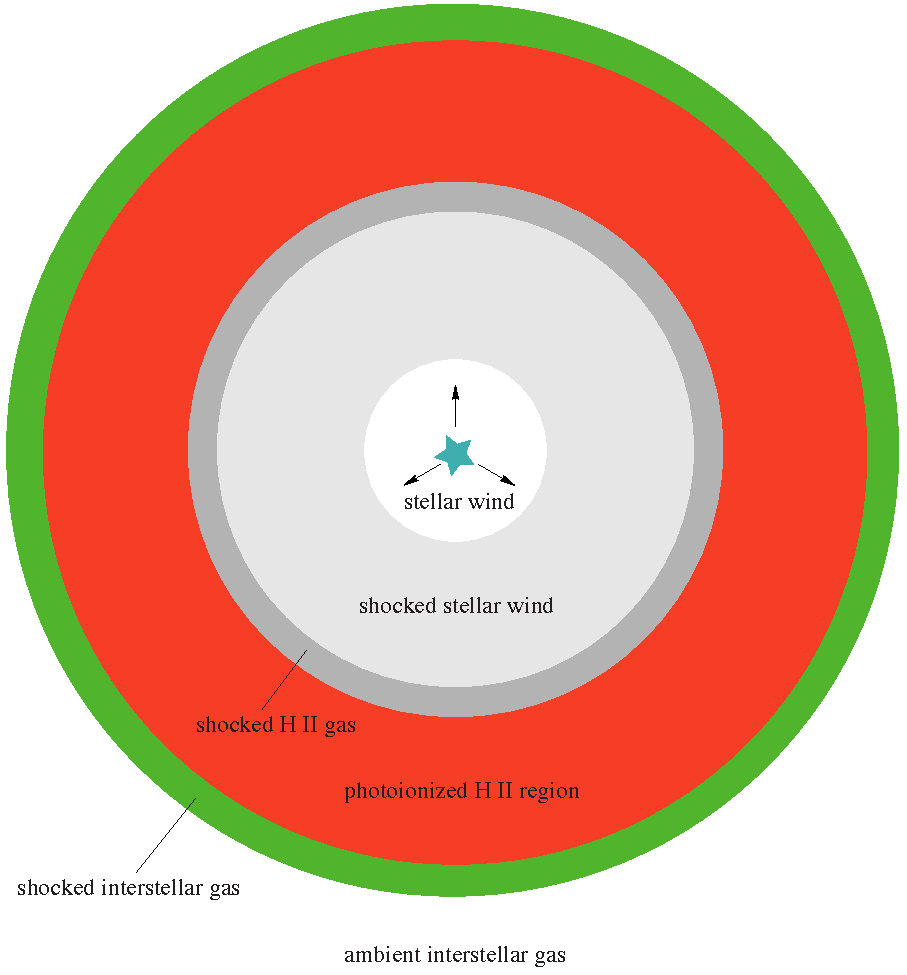
\includegraphics[width=3in]{schematic}
\caption{Schematic structure of a bubble, adapted from \citep{Freyer03}. The red and green colors encode the typical morphology seen in \emph{Spitzer} images, where green is assigned to 8 \um\, emission -- dominated by PAH fluorescence -- and red is assigned to 24 \um\, emission -- dominated by hot dust.}
\label{fig:schematic_ch6_brut}
\end{figure}

\begin{figure}[h!]
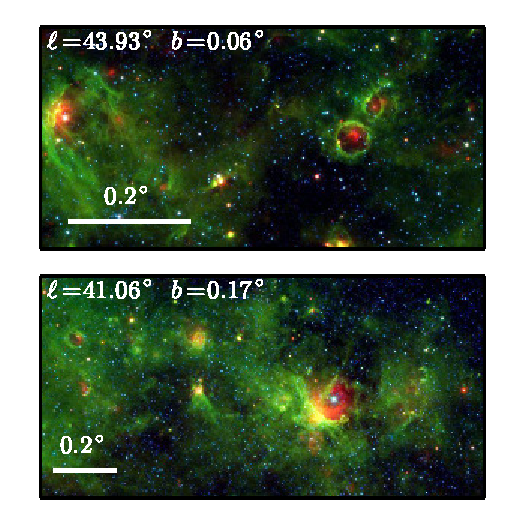
\includegraphics{mwp}
\caption{Example images presented to Milky Way Project citizen scientists to identify bubbles. The images show 4.5\um\, emission in blue,  8\um\, emission in green, and 24\um\, emission in red.}
\label{fig:mwp}
\end{figure}

\begin{figure*}
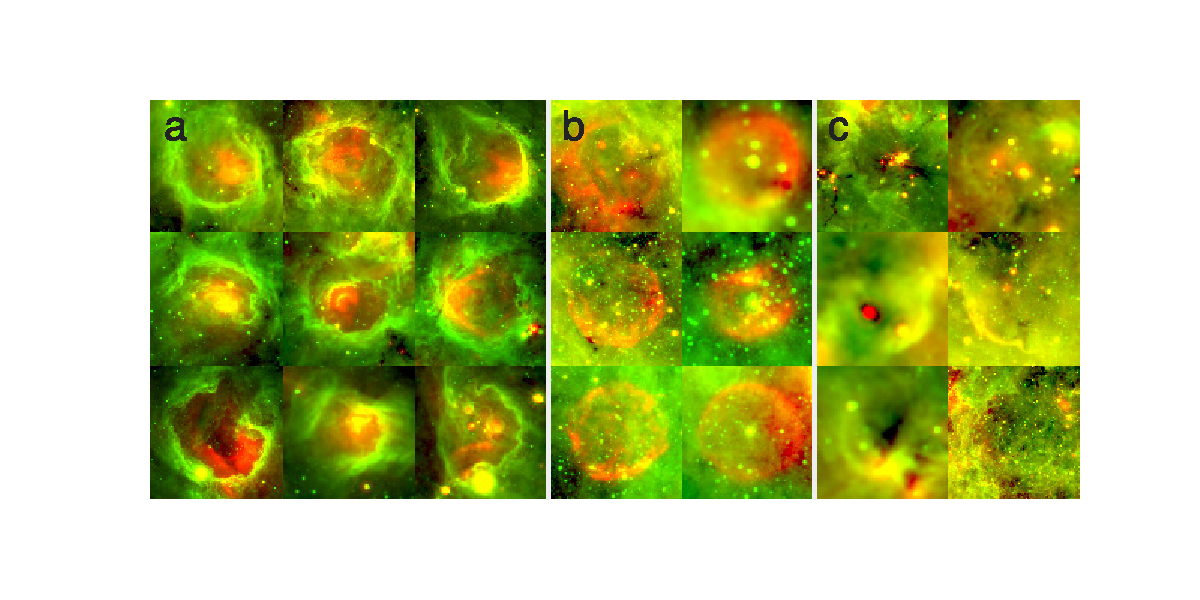
\includegraphics[trim= .7in 0 0 0, clip]{gallery}
\caption{Different astrophysical objects in the MWP catalog. a) ``Canonical'' wind-blown bubbles and \hii\, regions. b) shells
without 8 \um\, PAH emission (likely supernovae or bubbles around evolved massive stars). c) generic ISM structures of unclear astrophysical origin.}
\label{fig:gallery}
\end{figure*}

\subsection{Manual and Automatic Classification in Astronomy}
\label{sec:benefits}

In terms of accuracy, humans still outperform computers in most image-based pattern recognition tasks (e.g., \citealt{Zhang10}). Because of this, morphologically complex structures in the ISM (including supernova remnants, outflows, bubbles, \hii\, regions, molecular and infrared dark clouds, and planetary nebulae) are still traditionally cataloged manually. Human classification has several disadvantages, however.

First, human classification is time consuming, and people-hours are a limited resource. Even by enlisting large communities of citizen scientists, data from next generation surveys will be too large to search exhaustively. For example, the $>$ 35,000 citizen scientists of the Milky Way Project classified roughly 45 GB of image data from \emph{Spitzer}. Current and next-generation astronomical datasets are many thousands of times larger than this, suggesting tens of millions of citizen scientists would be needed for similar exhaustive searches through tera- and petabyte datasets.

Second, many scientifically important tasks are not suitable for enlisting the public. Part of the appeal of the Milky Way Project is due to the fact that the \emph{Spitzer} images are beautiful, contain many bubbles, and are compelling to browse through. Searches for very rare objects, or tasks where the scientific justification is less apparent to a citizen scientist, may be less likely to entice large volunteer communities. \cite{Raddick13} considers the motivations of citizen scientists in greater detail.

Finally, manual classification is not easily repeatable, and hard to calibrate statistically. For example, it is unknown how well the consensus opinion among citizen scientists corresponds to consensus among astronomers. The MWP catalog does not include any estimate of the probability that each object is a real bubble, as opposed to another structure in the ISM.

Automatic classifications driven by machine learning techniques nicely complement human classification. Such an approach easily scales to large data volumes and is immune to some of the factors that affect humans, like boredom and fatigue. Furthermore, because algorithmic classifications are systematic and repeatable, they are easier to interpret and statistically characterize. Despite the structural complexity of the ISM, \cite{Beaumont11} demonstrated that automatic classification algorithms can discriminate between different ISM structures based upon morphology.

The downside to automated classification for tasks like bubble detection is that the algorithms typically require a training set of example objects to classify. Fortunately, the Milky Way Project catalog provides just such a training set. We build an automatic bubble detector from these data in the present paper. There are several reasons to do this:

\begin{enumerate}
\item The automatic classifier is capable of producing quantitative reliability estimates for each bubble in the MWP catalog, potentially flagging non-bubble interlopers and leading to a cleaner catalog (Section \ref{sec:prob}).

\item We can search for bubbles not detected by MWP citizen scientists (Section \ref{sec:blind}).

\item We can treat this task as a case study for complex classification tasks in future datasets, where exhaustive manual classification will not be feasible (Section \ref{sec:next_steps}).
\end{enumerate}

\section{Classification Method}
\label{sec:method_ch6_brut}

Our goal is to use the set of citizen-scientist-identified bubbles to build an automatic detector that, when presented with a region of the sky in the  \textit{Spitzer} {\sc glimpse} and {\sc mipsgal} surveys, accurately determines whether or not the image contains a bubble. Our approach, which we name Brut, is an example of a supervised learning problem. Here is a brief overview of the task:

\begin{enumerate}
\item Build a representative training set of examples of bubble and non-bubble images. This will be derived from the MWP dataset.
\item Convert each example to a numerical \textit{feature vector} that describes each object, and captures the difference between bubbles and non-bubbles.
\item Feed the training data to a learning algorithm to build a model.
\item Use a subset of the examples not used during training to optimize the tunable parameters (so-called \textit{hyper-parameters}) of the learning algorithm.
\end{enumerate}

\subsection{Training Data}
\label{sec:method_training_data}
The MWP catalog is a natural choice for a training dataset. However, as shown in Figure \ref{fig:gallery}, the catalog as a whole contains many examples of objects that are not bubbles, and can compromise the training process. Thus, we manually curated a list of 468 objects in the Milky Way Project catalog which were clear examples of bubbles. We focus our attention on objects in the large bubble catalog, which contains 3744 out of 5106 total bubbles, with simimajor axes  $a \geq 13.5''$  \citep{Simpson12}. We focus on the large bubble catalog since the web interface used to build the small catalog was different, and may have different selection biases. The largest bubble in the MWP catalog has a semi major axis $a=10.3'$. This upper limit is set by the widest-field images presented to citizen scientists -- we discuss an implication of this cutoff in Section \ref{sec:prob}.

Training also requires an example set of non-bubbles. In principle, any random region of the sky that doesn't overlap an object in the MWP catalog is a candidate negative example -- while some of these fields actually contain bubbles not in the MWP catalog, they are rare enough that they don't  impact the training. However, we found that selecting negative examples at random was sub-optimal. The reason for this is that most random fields are nearly empty, and easily distinguished from fields with bubbles. Classifiers generated from such a dataset incorrectly labeled nearly any field containing ISM structure as a bubble.

A better set of negative examples includes more fields containing structure (Figure \ref{fig:bootstrap_neg}). We built such a collection in a bootstrapped fashion. Starting with random negative examples, we trained a classifier and used it to scan a large number (20,000) of negative fields. We then discarded half of the initial negative examples (those classified most confidently as not containing bubbles), and replaced them with a random sample of the mis-classified examples. We repeated this process several times, but found that one iteration was usually sufficient to build a good set of training data.

\begin{figure}[h!]
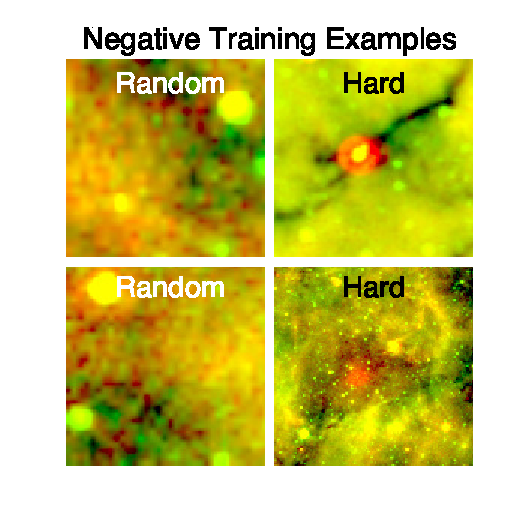
\includegraphics{bootstrap_neg}
\caption{Examples of typical randomly selected negative examples (left), and ``hard'' examples (right). Including more hard examples produces more discriminating classifiers.}
\label{fig:bootstrap_neg}
\end{figure}

\subsection{Feature Extraction}
\label{sec:method_feature_extraction}
Supervised classification algorithms distinguish between classes of objects based on numerical \textit{feature vectors} that summarize each object. Feature vector design is often the most important stage of supervised classification and, unfortunately, also the hardest. The ideal feature vector captures the differences between each class of objects, so that examples from different classes occupy different sub-regions of feature space.

In the case of image classification, the most obvious choice for a feature vector is simply the numerical value of the pixels themselves. This turns out to be a poor choice, because extended objects like bubbles are characterized by correlations between hundreds or thousands of pixels, and any individual pixel is virtually irrelevant to the classification task. Machine learning algorithms generally perform better when individual elements of the feature vector are more important to the classification, and less dependent on the value of other feature vector elements.

Our feature vectors have been designed based on insights in the automated face detection literature \citep{ViolaJones}.  The basic strategy is to encode a very large number ($\sim$40,000) of generic statistics about extended structures at various positions and scales. This strategy seems to be more effective than trying to tune a feature vector to the specific object being identified. While most elements in the feature vector will have no predictive power in the classification, the appropriate learning algorithm will simply ignore this information.

To construct our feature vector for a given region in the sky, we first extract a (40x40) pixel postage stamp of the field from IRAC 8 \um\, and MIPS 24 \um\, images. Following a scheme similar to \cite{Simpson12}, these images are intensity clipped at the 1 and 97th percentile, normalized to maximum intensity of 1, and passed through a square root transfer function. This scaling tends to do a good job of emphasizing ISM structure, making bubbles more visible to the eye. Then, the following properties were extracted from each postage stamp, and concatenated to form the feature vector:

\begin{enumerate}
\item The wavelet coefficients from the Discrete Cosine and Daub4 wavelet transforms. These coefficients encode how much power is in various spatial frequencies.
\item The image dot product\footnote{i.e., the sum of the pixel-by-pixel product of two images} of each image with 49 template images of circular rings of different size and thickness. Bubbles are morphologically similar to these templates, and presumably have larger dot products than a random intensity distribution.
\item The byte size of each compressed postage stamp image -- images substantially more or less smooth than a bubble compress to smaller and larger files, respectively.
\item The DAISY features of the image \citep{DAISY}. DAISY features are derived from measurements of local intensity gradients, and encode information about simple shapes in images; they are conceptually similar to edge detection filters.
\end{enumerate}

\subsection{Training}
While there are many algorithms designed to learn classifications form a training set of feature vectors, we focus here on the Random Forest algorithm \citep{Breiman01}. Random Forests are aggregates of a simpler learning algorithm called a decision tree. A decision tree is conceptually similar to the game twenty questions: in this game, one player asks a series of yes/no questions in an attempt to deduce the identity of a hidden object selected by another player. Likewise, a decision tree classifies an object by performing several boolean tests on elements of that object's feature vector (e.g., $F_3 > 5$). These tests are arranged in a binary tree. The decision tree algorithm traverses this tree for each object, traversing the left or right subtree depending on whether each boolean test is True or False. The leaves of the tree contain the final classification (in the present context, ``bubble'' or ``not bubble'').

The decision tree is constructed from the training data, where the feature vectors and classification are both known. Trees are built one node at a time, in a greedy fashion -- that is, at every step of the learning process, a node is added to the tree to maximize the tree's classification performance on the training data. Several different heuristics can be used to measure classification performance.

On their own, decision trees are prone to over-fitting the training data by adding too many nodes. In a more traditional fitting context, this is analogous to adding too many terms to a polynomial fit of noisy data -- in both situations, the model describes the input data very well, but does not generalize to new predictions. Random Forests overcome this problem by building several trees on different subsets of the data. Since over-fitting is sensitive to the exact input data used, each individual tree in a Random Forest over-fits in a different way. By averaging the classifications of each tree, the Random Forest mitigates over-fitting. Random Forests have proven effective in many machine learning contexts \citep{Kuhn13}.

In addition to good performance and robustness against over fitting, the Random Forest algorithm has several other advantageous properties: it is possible to interpret how important each element in the feature vector is to the classification, the algorithm naturally ignores irrelevant elements of the feature vector, and it is conceptually and computationally simple.

\subsection{Hyperparameter Optimization}
The Random Forest algorithm has a small number of tunable parameters. The most important of these are the number of trees in the forest, and the heuristic used to measure classification quality when building each tree. We determined good settings for these ``hyper-parameters'' using cross validation. During cross validation, the training data is partitioned into two sets. The model is fit to the first set using a given set of hyper-parameters, and is evaluated on the second set. This process repeats for each combination of hyper-parameters, and the combination with the best performance on the test data is used for the final model. From our cross-validation analysis, we chose forests with 800 trees, using the information gain heuristic \citep{Raileanu04}.

\subsection{Final Model}

Classifiers cannot be used to re-classify the data used to train them, due to the possibility of over-fitting. Thus, to obtain valid classifications for all fields, we constructed three classifiers. Each classifier was trained using data from two-thirds of the sky, and used to classify the remaining third. The three training zones are interleaved longitude sections, so that each classifier is sensitive to trends with longitude. Figure \ref{fig:zone} depicts how the $0 < \ell < 10$ region is partitioned -- the shaded regions denote the portion of the sky used to train each classifier. The three classifiers are identical apart from the longitude zones used for training and classification.

\begin{figure}[h!]
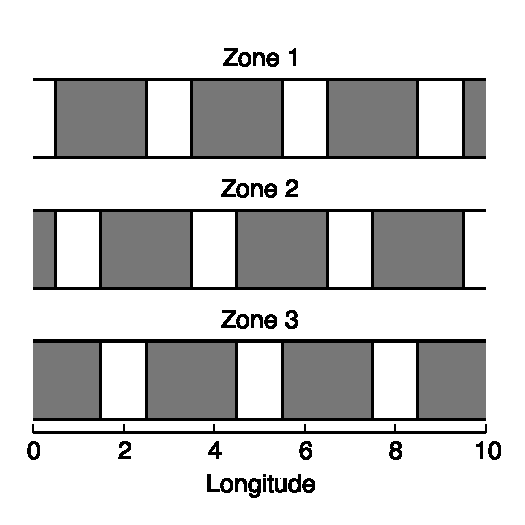
\includegraphics{zones}
\caption{Illustration of the zones used to train each classifier. Each classifier is trained using the data from the shaded regions in its zone, and used to classify the light regions.}
\label{fig:zone}
\end{figure}

\subsection{Using the classifier}

The output from Brut is a score between -1 and 1, which is directly proportional to the fraction of trees in the forest which classify a feature vector as a bubble. This score provides more information than a simple binary classification, as it gives some sense of the confidence of the classification. Furthermore, one can adjust the threshold that defines when an object is considered to be a bubble. Increasing the threshold increases the reliability of the catalog, at the cost of completeness.

One standard way to summarize the performance of a classifier is to plot the false positive rate (fraction of negative examples incorrectly classified) versus the true positive rate (fraction of bubbles correctly classified) as the threshold varies. This is called the Receiver Operating Characteristic, and is shown for the three classifiers in Figure \ref{fig:roc}. The false positive rate is measured by classifying $\sim 15000$ random negative fields, and the true positive rate is measured using the high-quality subset of the MWP catalog described above. Recall that the set of bubbles in this test set were selected because they are very well defined. Thus, Figure \ref{fig:roc} overestimates the true positive rate when presented with more ambiguous bubbles. We compare the performance of the classifier on more representative bubbles in Section \ref{sec:expert}.

\begin{figure}[h!]
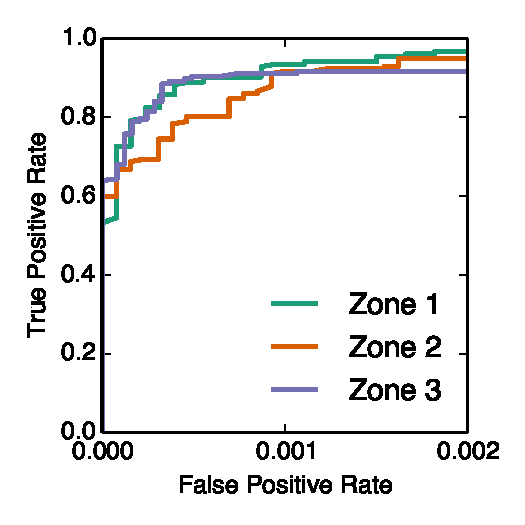
\includegraphics{roc}
\caption{The tradeoff between false positive rate and true positive rate, for the three classifiers in Brut. Each classifier is trained using a different zone, depicted in Figure \ref{fig:zone}.}
\label{fig:roc}
\end{figure}


\subsection{Building a Catalog}
\label{sec:build}

Using our automatic bubble classifier to conduct a full search for bubbles in \textit{Spitzer} data is straightforward. The main task involves scanning the classifier over all images, at all scales. At each of these regions, the classifier yields a score, representing its confidence that the field contains a bubble. A simple threshold on this score identifies regions likely to contain a bubble -- from the discussion of Figure \ref{fig:roc} above, adjusting this threshold sets the tradeoff between completeness and reliability. Note that Brut only attempts to determine the location and size of bubbles. Citizen scientists, on the other hand, were able to constrain the aspect ratio, position angle, and thickness of each object.

In practice, the classifier is insensitive to small adjustments to the size or location of the field. As a result, bubbles are usually associated with a cluster of regions that rise above the detection threshold (the white circles in Figure \ref{fig:cluster}). We follow a simple procedure to merge these individual detections. Given a collection of raw detections, this procedure identifies the two nearest locations at similar scales, and discards the location assigned a lower score by the classifier. This process repeats until no two fields are close enough to discard. Two fields are close enough to merge if they are separated by less than the radius of either field, and have sizes that differ by less than 50\%. The red circle in Figure \ref{fig:cluster} shows the result of merging detections.

\begin{figure}[h!]
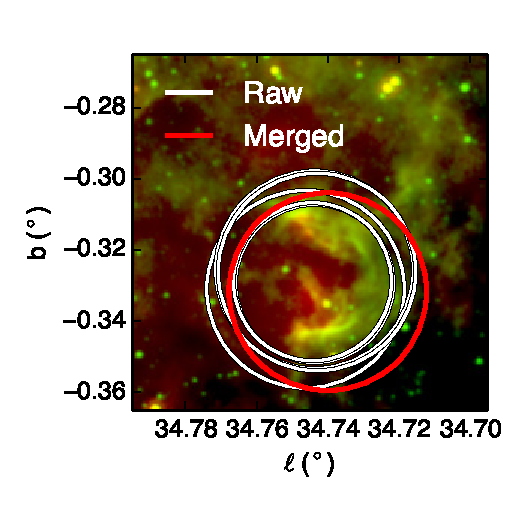
\includegraphics{cluster}
\caption{An illustration of how Brut merges multiple bubble detections. Each white circle is a location with a high Brut score. The red circle is the region with the highest brut score, and is used as the final detection.}
\label{fig:cluster}
\end{figure}

This practice works well for isolated bubbles, but occasionally fails for bubble complexes with multiple, overlapping bubbles. A more sophisticated clustering analysis may well perform better in this situation.

\section{Expert Validation}
\label{sec:expert}

To evaluate the performance of Brut, we need a set of ``ground truth'' classifications. However, to some extent identifying bubbles in \textit{Spitzer} images is inherently subjective. While the objects in Figure \ref{fig:gallery}a are unambiguously associated with star formation, other sources are not. In some cases -- particularly irregular bubbles, or those with faint or no 24\um\, emission -- it is unclear whether cavities seen in 8 \um\, data are actively sculpted by young stars, or merely the underlying structure of the undisturbed ISM.

The subjectivity of bubble identification has received only limited attention. The MWP catalog includes a ``hit rate'' measurement that lists the fraction of citizen scientists who identify a specific bubble, relative to the total number of users who viewed an image containing that bubble. However, as discussed above, the Milky Way Project catalog contains many objects besides bubbles. Thus, while the hit rate communicates how visually salient a particular ISM feature appears to MWP users, it does not directly convey how much consensus astronomers have about the astrophysical nature of that feature.

To better measure the level of expert consensus in bubble identification, we conducted a small online survey. The astronomer participants of this survey were presented with a sequence of 92 \emph{Spitzer} images at three zoom levels and two contrast settings. They were asked to assign each image to one of three categories: clear examples of bubbles or \hii\, regions, ambiguous or irregular bubbles, or Non-bubbles. Appendix A discusses the survey setup in more detail.

\subsubsection{Validation of the Milky Way Project Catalog}
\label{sec:expert_mwp}
Of the 92 images in the expert survey, 45 were a random subset of objects in the MWP catalog (the remaining fields are discussed in the next section). Figure \ref{fig:expert_mwp_votes} shows the voting breakdown for these objects. Each row corresponds to a single object, and the red, orange, and blue bars show the fraction of experts who classified the image in each category.  We call attention to several aspects of this distribution:


\begin{figure}[h!]
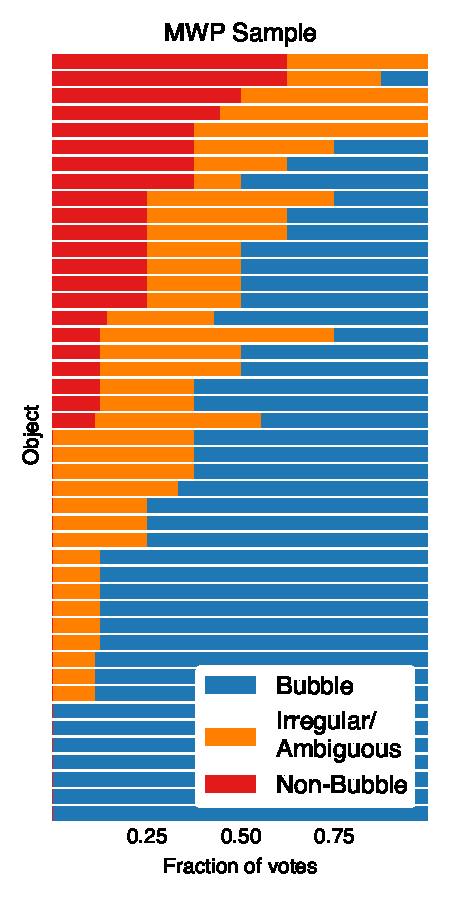
\includegraphics{expert_mwp_votes}
\caption{The distribution of expert classifications for 41 objects in the Milky Way Project bubble catalog. Each row corresponds to an image, and the colored bars in that row indicate the fraction of experts who categorized the image as a Bubble (blue), Irregular or Ambiguous Bubble (orange), and Non-Bubble (red).}
\label{fig:expert_mwp_votes}
\end{figure}

\begin{enumerate}
\item Only 15\% of these objects -- 7 out of 41 -- were unanimously classified as clear bubbles -- this number increases to about 50\% if all irregular and ambiguous objects are optimistically treated as bubbles.
\item Depending on how many irregular/ambiguous objects are bubbles, between 10 and 30\% of objects in the MWP catalog are judged by experts to be interlopers -- that is, objects which are unlikely to be the result of a young star sculpting the surrounding ISM. While some of these regions might be other interesting astrophysical objects like supernova remnants, most appear to be incidental, non-dynamical structure in the ISM.
\item The most popular category for each object is chosen by 70\% of experts on average. In other words, when using \emph{Spitzer} images, determining the ``true'' nature of a typical object in the MWP catalog is subjective at the 30\% level. Citizen scientists, by comparison, exhibit much lower levels of agreement; the average hit-rate for these objects is 0.2.
\end{enumerate}

Is it possible to determine which of the remaining objects in the MWP catalog would likely be rejected as interlopers by experts? The hit rate of each object in the catalog might correlate with expert opinion, and be a useful filter. Likewise, the confidence score computed by Brut might identify interlopers. Figure \ref{fig:expert_mwp_score} plots the citizen's hit rate and Brut's confidence score compared to the expert classification. The Y position of each point denotes the level of consensus for each object -- the percentage of experts who chose the plurality category. Both metrics partially separate bubbles from the other categories. The hit rate is more effective at penalizing orange and red objects, which are confined to hit rate $<0.2$ in panel a. On the other hand, the hit rate is ineffective at isolating bubbles with high expert consensus. The Brut score is more effective at identifying these high-consensus bubbles, which is apparent by the cluster of blue points in the upper right corner of panel b. We also plot in Figure \ref{fig:expert_mwp_score}c a joint score -- the sum of the normalized and mean-subtracted Brut score and hit rate.  This combines the strengths of the individual metrics, and achieves the best separation.

\begin{figure*}
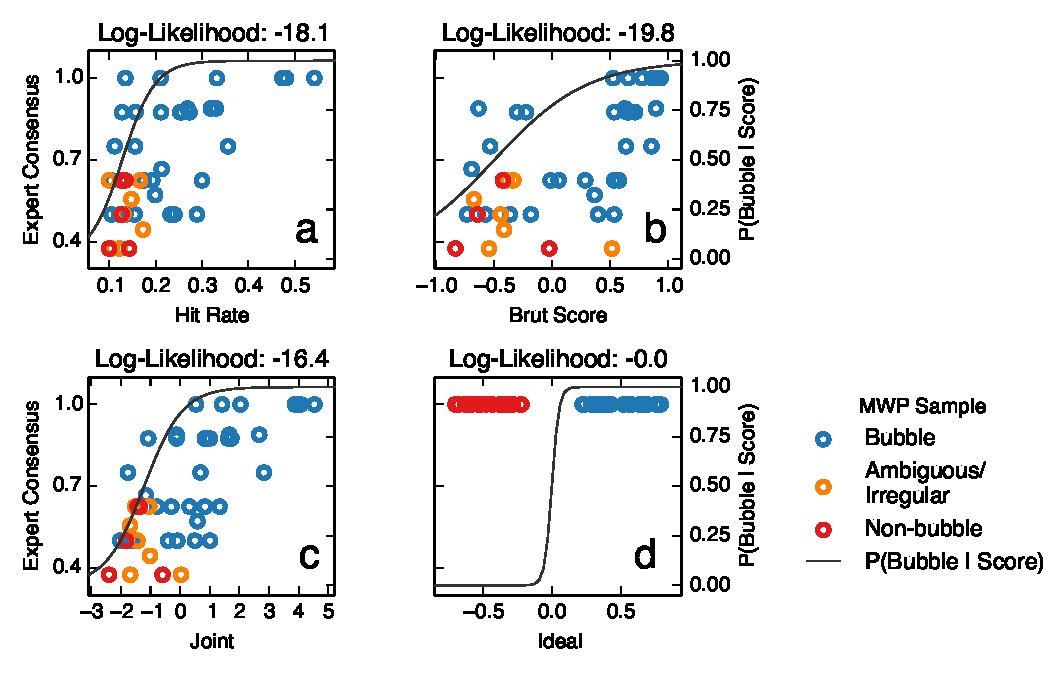
\includegraphics[width=6in]{expert_mwp_score}
\caption{The ability for the MWP hit rate and Brut score to predict expert expert classifications for objects in the MWP catalog. Each circle represents an object in the MWP catalog. Color depicts the most popular classification, and the y-position indicates the fraction of experts who chose this category. The curves estimate the bubble probability (right Y axis), obtained via logistic regression to the object category. The Joint metric, which combines the Hit Rate and Brut score, is best able to predict expert classifications. The title reports the log-likelihood of each logistic fit, according to Equation \ref{eq:likelihood}. Panel d depicts the ideal situation, where classes are unambiguous.}
\label{fig:expert_mwp_score}
\end{figure*}

The expert reclassifications of this sample of Milky Way Project objects can be used to convert a raw score like the joint score to a calibrated probability that an expert would classify an object as a bubble, given that score. To achieve this, we perform a logistic regression against each of the three scores (hit rate, Brut score, and joint score). The logistic regression only considers whether the plurality category for each object is a bubble -- the consensus information is not used. The grey curves in Figure \ref{fig:expert_mwp_score} trace this curve, and show the predicted probability that an object is a bubble given the score on the X axis. We reiterate that this is \emph{not} a fit through the (X, Y) cloud of points in the plot; rather, it is (informally) a fit to the fraction of circles which are blue at each X location of the plot. The title of each panel reports the quality of each fit, as defined by the log-likelihood:

\begin{equation}
\mathcal{L} = \sum_{\rm Bubbles} \log\left(P\left({\rm Bubble | Score}\right)\right) + \sum_{\rm Non-Bubbles} \log\left(1 - P\left({\rm Bubble | Score}\right)\right)
\label{eq:likelihood}
\end{equation}

Panel d in Figure \ref{fig:expert_mwp_score} shows the ideal situation, where a scoring metric perfectly separates two classes of unanimously-categorized objects. The joint score combines the information from citizen scientists and Brut, and comes closest to this ideal. While the logistic curves for the hit rate and joint score look similar, the latter curve is a better fit to the data as judged by the higher likelihood of the data under this model.

\subsubsection{Uniform Classification}
The remaining 47 regions in the expert survey were selected randomly from the full set of fields analyzed during Brut's full scan of the \emph{Spitzer} images. A fully random sample from this collection is uninteresting, since the majority of fields are blank areas of the sky. Instead, these 47 images are approximately uniformly distributed in the Brut confidence score. We refer to these images as the ``uniform'' sample.

The expert vote distribution for these images is shown in Figure \ref{fig:expert_uniform_votes}. There are more non-bubble fields in this sample, but the overall properties are otherwise similar. The average field is classified with a 72\% consensus.

Figure \ref{fig:expert_uniform_score} shows the Brut score for each field in the uniform sample, compared to the plurality category (color) and level of consensus (Y axis). The Brut score does a good job of separating the high consensus objects. Overall, however, the classes overlap more for the uniform sample than for the MWP sample. This is also expected, since all objects in the MWP sample have been previously identified by citizen scientists as potential bubble sites. The uniform sample does not benefit from this information, and is representative of the harder, ``blind'' classification task. As before, a logistic fit can be used to estimate, for objects identified in a blind search, the probability of being a bubble given the Brut score.

\begin{figure}[h!]
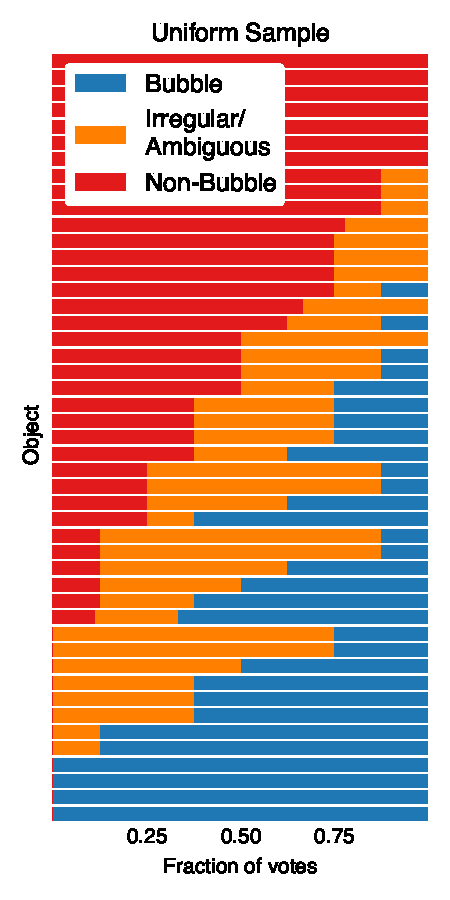
\includegraphics{expert_uniform_votes}
\caption{The same as Figure \ref{fig:expert_mwp_votes}, for the Uniform sample.}
\label{fig:expert_uniform_votes}
\end{figure}

\begin{figure*}
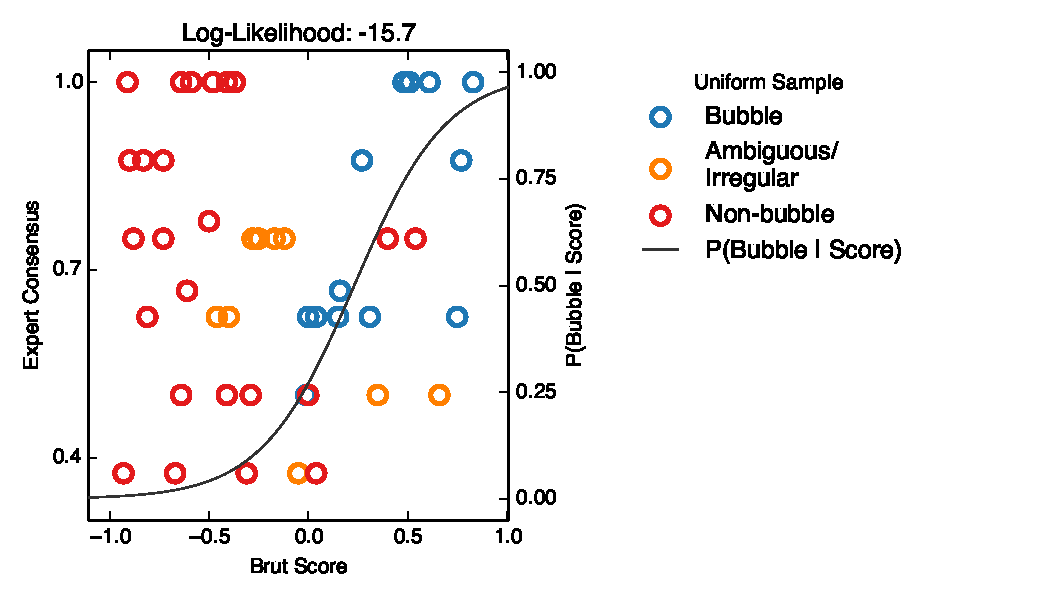
\includegraphics{expert_uniform_score}
\caption{The same as Figure \ref{fig:expert_uniform_score}, for the Uniform sample.}
\label{fig:expert_uniform_score}
\end{figure*}

\section{A Probabilistic Bubble Catalog}
\label{sec:prob}
Section \ref{sec:expert_mwp} outlines a strategy to combine hit rates with Brut's own confidence score to predict whether or not
an expert would classify each object in the original MWP catalog as a bubble. We have assigned a bubble probability to each
object in MWP catalog based on this analysis (Table \ref{table:prob_table_ch6_brut}). The high-probability subsample of this catalog displays several interesting differences compared to the unfiltered catalog.

To explore the differences between the high and low reliability portions of the MWP catalog, we have split the catalog into three roughly equally-sized groups: those where $P_{\rm bubble} < 0.5$, $0.5 < P_{\rm bubble} < 0.9$,
and $P_{\rm bubble} > 0.9$. Figure \ref{fig:dist_lon} shows the longitude distribution for each of these groups. The distributions are mostly similar, except at the three longitudes marked with vertical lines. These longitudes exhibit an excess of low-probability bubbles relative to the other groups.  All three fields are in fact sites of large, degree-scale giant \hii\, regions -- two are shown in Figure \ref{fig:wide_fields}.

The excess of low-probability objects towards $\ell=-43^\circ$ coincides with a large bubble complex, containing bubbles S108-S111 in \cite{Churchwell06}. The region at $\ell=-55^\circ$ coincides with the Dragonfish nebula, studied by \cite{Rahman11}. Finally, the $\ell=-62^\circ$ region contains the G305 star forming complex studied by \cite{Hindson12}.

To determine whether the overabundance of low-probability sources near giant \hii\, regions indicates a failure of the probabilistic scoring or a bias in citizen scientist annotations, the lead author manually inspected the objects in the $\ell=-61^\circ$ bin. The sum of bubble probabilities for the 25 MWP objects in this bin is 8.09, and implies that an expert would identify $\sim 8$ of these objects as real bubbles if the probabilistic score is correct. Roughly 5-6 of these objects are compelling bubble candidates, which suggests that the excess of low-probability bubbles is not due to an overly conservative scoring strategy. Instead, this points to a real citizen scientist bias towards over-identification of bubbles in active regions like this. The central source in each of these regions creates a large, complex cavity in the ISM, and fluoresces much of the surrounding material as well. This leads to an abundance of coincidental, arc-like features misidentified as bubbles. The scores provided by Brut are able to identify this problem, and exclude the interlopers.

While citizen scientists are prone to over-identify bubbles towards giant \hii\, regions, they are unlikely to identify these large regions themselves. This might be because such objects are to irregular, or simply too big to see well in any single image served during the Milky Way Project. The widest zoom levels at which Brut scans through image data is wider than the widest images seen by citizen scientists, and it recovers some of these regions. For example, Figure \ref{fig:wide_fields} shows in magenta the new regions which Brut scores $>0.2$ on a blind search, that have no match in the MWP catalog. Each panel includes a new detection that is bigger than the biggest previously-cataloged objects. Still, Brut does not identify the large \hii\, regions themselves as bubbles. This is partially due to the fact that these large bubbles are absent from the MWP catalog, and thus Brut was never ``taught'' that objects like these should be considered bubbles.

In discussing the longitude distribution of bubbles, \cite{Simpson12} noted a dip in bubble counts at $|\ell| < 10^\circ$. They postulated that this might be because confusion in this busier region makes identification more difficult. However, this dip is most apparent for low-probability objects. In other words, the dip in the longitude distribution is not driven by a decrease in completeness, but rather by an increase in reliability. Perhaps, due to the complex background of emission towards the Galactic center, citizen scientists were less likely to notice subtle, coincidentally arc-like structures in the ISM.

\begin{figure}[h!]
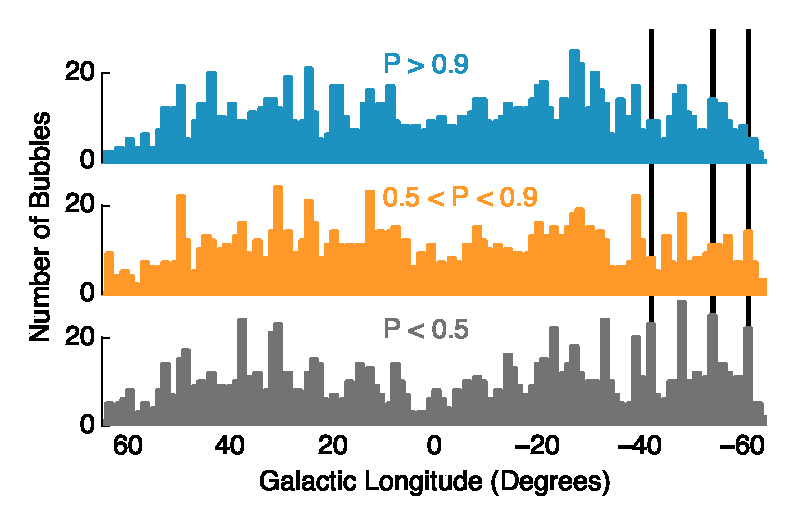
\includegraphics{dist_lon}
\caption{The longitude distribution for the MWP catalog, partitioned according to the bubble probability score.
Vertical black lines identify three degree-scale emission complexes with an overabundance of low-probability objects.}
\label{fig:dist_lon}
\end{figure}


\begin{figure*}
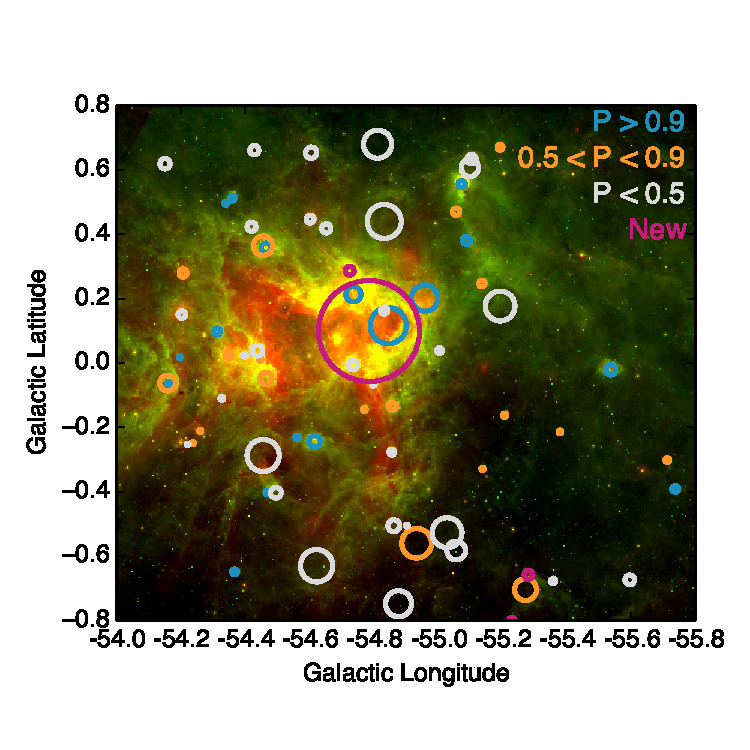
\includegraphics[trim=0 .3in 0 .6in, clip]{l305}
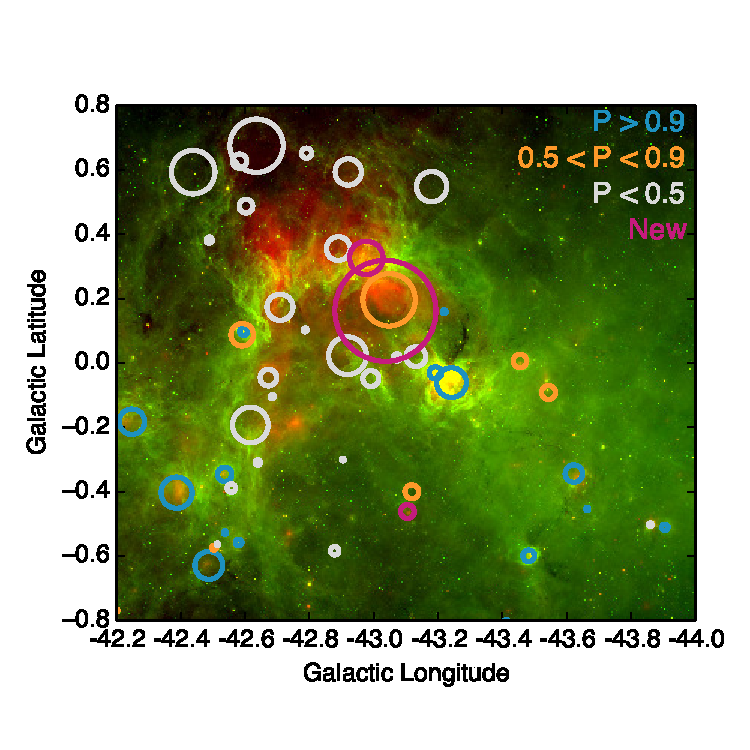
\includegraphics[trim=0 .3in 0 .6in, clip]{l317}
\caption{Two fields with overabundances of low-probability bubbles in the MWP catalog.}
\label{fig:wide_fields}
\end{figure*}

Figure \ref{fig:dist_lat} shows the latitude distribution for each subsample. The lowest-probability objects display a slightly broader distribution, particularly evident at $|b| > 0.5^\circ$. Because the ambient intensity field falls off quickly away from the mid-plane, we suspect random arc-like ISM structures are more likely to catch the eye in these regions.

\begin{figure}[h!]
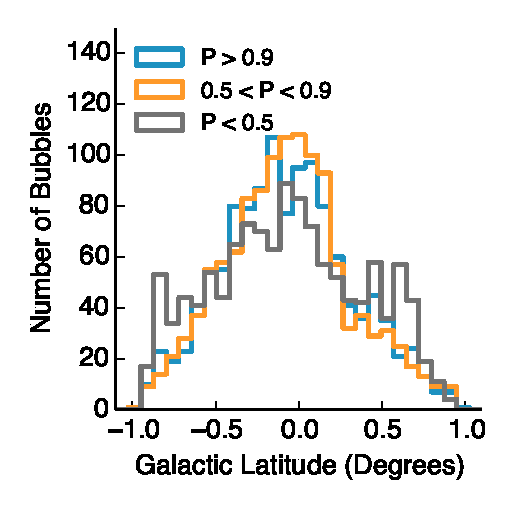
\includegraphics{dist_lat}
\caption{The latitude distribution for the MWP catalog, partitioned according to the bubble probability score.
Low-probability objects have a slightly wider distribution.}
\label{fig:dist_lat}
\end{figure}

Of the 3661 objects with bubble probability scores, 126 coincide spatially with \hii\, regions from \cite{Anderson11}. As Figure \ref{fig:hii_score} shows, objects associated with these \hii\, regions are strongly skewed towards higher bubble probabilities. This correlation strengthens the argument that the probability score successfully identifies dynamical objects.

\begin{figure}[h!]
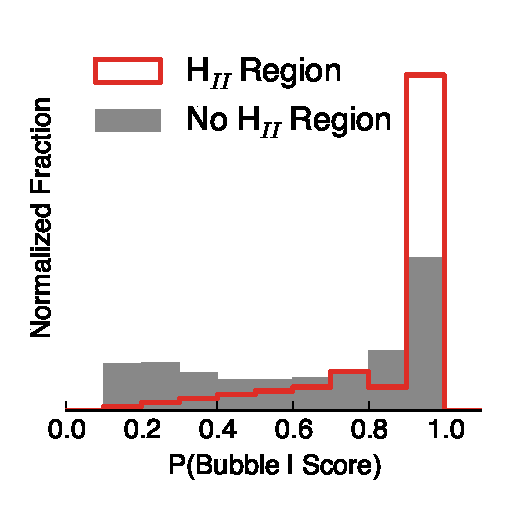
\includegraphics{dist_hii_score}
\caption{The bubble probability distribution for sources with and without \hii\, region counterparts in the \cite{Anderson11} catalog.}
\label{fig:hii_score}
\end{figure}

\cite{Anderson11} reports disambiguated kinematic distances for the \hii\, regions in their catalog. Figure \ref{fig:dist_map} shows the position and sizes of the 128 bubbles associated with \hii\, regions with known distances, overlaid on a schematic map of the Galaxy's spiral structure. Four of the low-probability objects associated with \hii\, regions have large angular and linear diameters. However, from manual inspection none of these regions are compellingly associated with a real bubble in the image data. Thus, their match to \hii\, regions seems to be coincidental and arbitrary.

While bubbles cluster around the Sagittarius arm, there are two clusters of bubbles in inter-arm regions -- one beyond the outer arm, and another apparent stream of bubbles around 5kpc, from $30^\circ < \ell < 60^\circ$. A bubble is a broad observational definition that covers several astrophysical phenomena, including \hii\, regions, non-ionized cavities from B star winds, and supernova remnants. Bubbles located on or between spiral arms may well correspond to different astrophysical classes or evolutionary stages. Furthermore, the detectability of bubbles is a complicated mixture of an object's size and brightness as a function of time, as well as the amount of unrelated structure along the line of sight to each object. Population synthesis studies which simulate realistic galactic environments and predict distributions akin to Figure \ref{fig:dist_map} might be able to constrain the relative mixture -- and dynamical importance -- of different classes of bubbles \citep{Robin03,Robitaille12}.

\begin{figure}[h!]
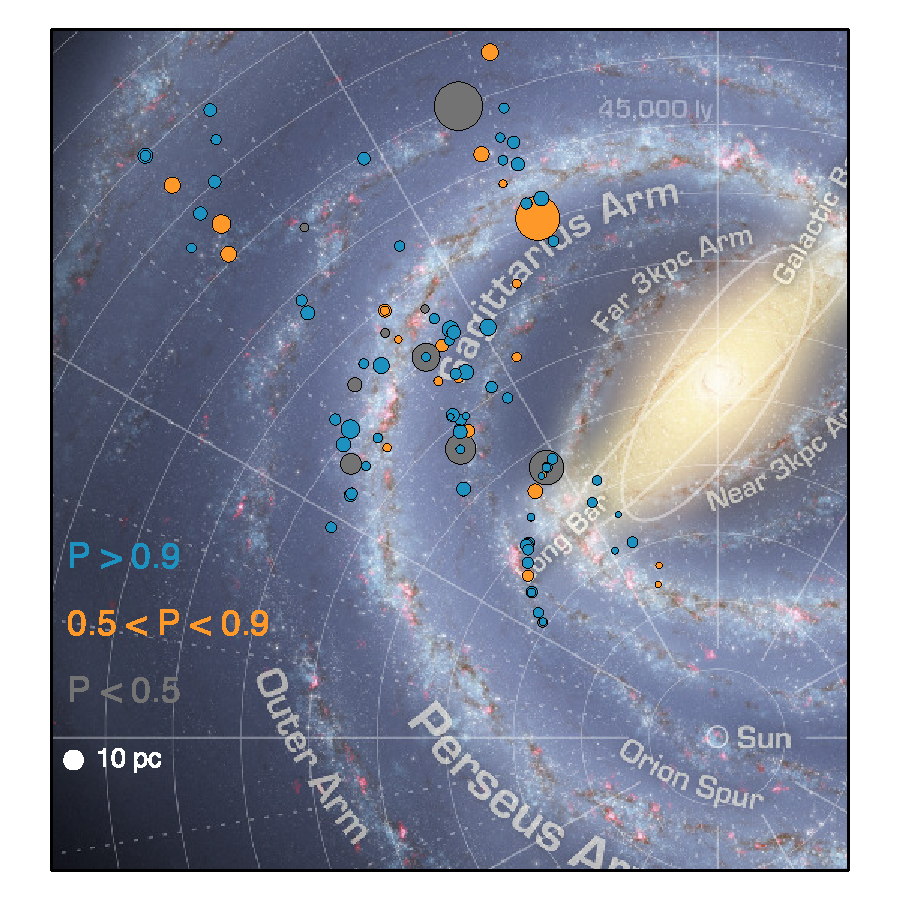
\includegraphics{dist_map}
\caption{Positions and sizes of bubbles with kinematic distance measurements from \cite{Anderson11}. The background image is an artist's schematic rendition of the Galaxy's spiral structure (credit NASA/JPL-Caltech/R. Hurt)}
\label{fig:dist_map}
\end{figure}

\subsection{Evidence for Triggering}

Bubbles are frequently studied in the context of triggered star formation. The material excavated by bubble-blowing stars might induce subsequent generations of star formation. Two main mechanisms for triggered star formation have been proposed: in the collect and collapse model \citep{Whitworth94, Dale07}, material gathered along bubble rims eventually passes a critical density and undergoes gravitational fragmentation and collapse. In the radiatively-driven implosion model, the wind or ionization shock front collides with pre-existing but stable cores, and the resulting compression triggers collapse \citep{Bertoldi89}.

In any particular region, finding clear evidence for triggered star formation is difficult. The typical approach is to identify an overdensity of young stars within or on a bubble rim, and/or to look for an inverse age gradient with bubble radius \citep{Deharveng05, Zavagno06, Koenig08}. Such an analysis is often confounded by small numbers of YSOs and ambiguous line-of-sight distances and stellar ages. Furthermore, it is often unclear whether spatial correlations between bubbles and YSOs imply a triggered relationship between the two, since star formation is a naturally clustered process \citep{Lada03}.

Such problems can partially be addressed by correlating YSOs with large bubble catalogs like the MWP catalog -- this does not disambiguate correlation from causation, but it can overcome problems related to small-number statistics. \cite{Thompson12} first applied such an analysis using the \cite{Churchwell06} catalog, and \cite{Kendrew12} later repeated this on the MWP catalog. This analysis computes an angular correlation function \citep{Landy93, Bradshaw11}, defined by

\begin{equation}
w(\theta) = \frac{N_{BY} - N_{BR_Y} - N_{R_BY} + N_{R_BR_Y}}{N_{R_BR_Y}}
\label{eq:corr}
\end{equation}
where $N_{\alpha \beta}$ represents the number of pairs of objects from catalogs $\alpha$ and $\beta$ with a separation of $\theta$, $B$ is a bubble catalog, $Y$ is a YSO catalog, and $R_B$ and $R_Y$ are randomly-distributed bubble and YSO catalogs. These random locations are chosen to preserve the approximate latitude and longitude distribution of each class of objects, but are otherwise uniformly distributed. Informally, $w(\theta)$ represents the excess likelihood of finding a YSO at a particular distance $\theta$ from a bubble, relative to what is expected from a random distribution of bubbles and YSOs. We normalize the angular offset $\theta$ by the radius of each bubble, such that $w(\theta)$ traces the excess YSOs as a function of offset in bubble radii. An ideal signature of triggered star formation, then, would be a local maximum of $w(\theta)$ at $\theta = 1$.

We reproduce the Figure 15 of \cite{Kendrew12} in Figure\ref{fig:trigger}a. This shows the angular correlation function between the Milky Way Project Large catalog and RMS catalog of YSOs and compact \hii\, regions \citep{RMS}, as a function of normalized bubble radius. The main signal is a decaying correlation, indicative of the fact that star formation occurs in clustered environments. The prediction from triggered star formation is that there should be an additional peak at $\theta \sim 1$ bubble radius. Such a signal is not obvious in this figure, though \cite{Kendrew12} report evidence for a peak for the largest bubbles in the MWP catalog. Likewise, \cite{Thompson12} report a clearer peak when considering the expert-selected bubbles in \cite{Churchwell06}.

In Section \ref{sec:expert}, we demonstrated that roughly 30\% of objects in the MWP catalog are interlopers -- random ISM structures incorrectly tagged as bubbles. Furthermore, the relative false positive rate increases towards giant \hii\, regions -- precisely the regions where one might expect triggered star formation to be most apparent. Interlopers might significantly dilute bubble/YSO correlations in the MWP catalog. Fortunately, our bubble probability scores allow us to identify many of these interlopers, yielding a higher reliability catalog that still has 3x as many bubbles as used by \cite{Thompson12}.

Figure \ref{fig:trigger}b shows the same correlation function, for the subsamples partitioned by bubble probability. This reveals an additional excess from $0.5 < \theta < 1$ bubble radius, whose strength increases with bubble probability. This is similar to the trend with bubble size that \cite{Kendrew12} reported, but the signal here is both stronger and due to a different subsample of bubbles -- the size distribution of bubbles does not vary significantly between the three probability bins.

Star formation is a naturally clustered process. The curves in Figure \ref{fig:trigger} trace the excess of RMS YSOs near bubbles relative to a purely random distribution of objects -- they do not measure the excess density of YSOs relative to other star formation regions. The red ``Control'' curve in Figure \ref{fig:trigger} addresses this. This curve was obtained by repositioning each bubble to the location of a random RMS YSO, and re-running the analysis. In other words, the curve shows the natural clustering of YSOs relative to each other. The left-most point of the curve is very large, which is an artifact of the fact that each bubble lines up exactly with the YSO it was repositioned to -- this creates a strong overdensity at very small $\theta$. Beyond this point, however, the curve resembles the $P < 0.5$ subset. The fact that the $P > 0.9$ bubbles fall significantly above the control curve indicates that YSOs are clustered around high-probability bubbles even more strongly than they cluster around one another on average. However, this clustering analysis cannot determine whether the overdensity around $P > 0.9$ bubbles is the result of bubble-triggered star formation, or rather an indication that bubbles form in particularly active star forming regions.

\begin{figure}[h!]
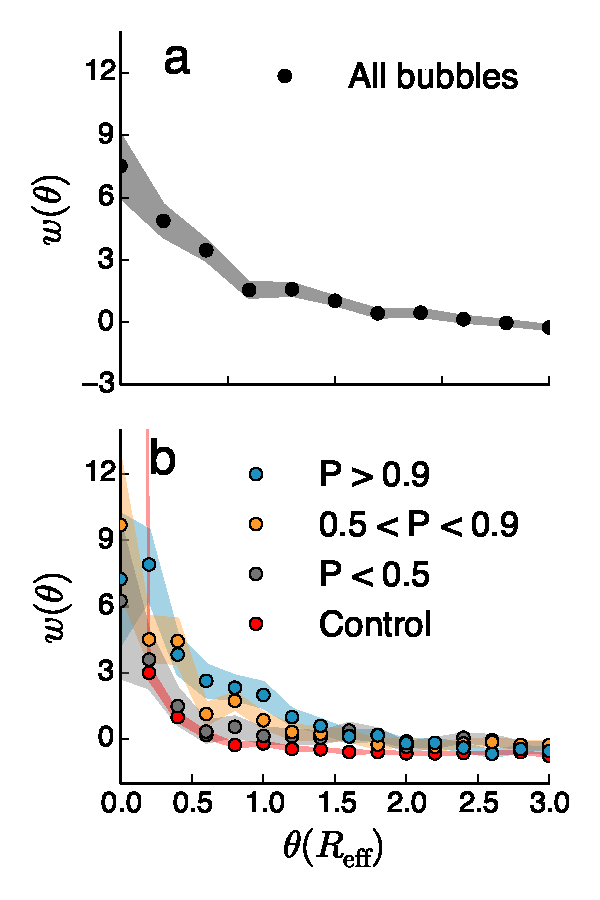
\includegraphics[width=3.1in]{trigger}
\caption{Angular correlation function (Equation \ref{eq:corr}) between bubbles and sources in the RMS catalog of YSOs. Error estimates (shading) are derived via bootstrap resampling from the bubble catalog. Top: the correlation function for all bubbles. Bottom: the correlation function for the
low (black), medium (orange), and high-reliability bubbles (blue). The red control curve is obtained by repositioning each bubble to coincide with a random YSO -- it measure the general clustering of YSOs.}
\label{fig:trigger}
\end{figure}

\section{Blind Search}
\label{sec:blind}
The previous section focused on using Brut to reassess bubbles previously identified by citizen scientists. We've demonstrated that Brut is successful at identifying the high-reliability subset of the MWP catalog and, conversely, at flagging probable interlopers in the catalog. The result is a purer statistical sample of bubbles in the Milky Way.

Now we consider the possibility of finding bubbles missing from the MWP catalog. By scanning through all {\sc glimpse}/{\sc mipsgal} data, Brut can be used to conduct a blind search for new bubbles. Discovering bubbles without knowing the citizen-science hit-rate at each location is a harder task; Brut does not benefit from complementary information about how citizen scientists classify a particular region. However, this task is relevant to future projects where machine learning techniques assist manual search. For applications where exhaustive human search is infeasible, machine learning algorithms can conduct exhaustive searches and flag interesting candidate objects for human attention or followup observation.

We performed a blind search with Brut as follows: starting at a minimum field of view of 80'', we scanned the entire {\sc glimpse}/{\sc mipsgal} survey area of $|\ell| < 65^\circ$, $|b| < 1^\circ$. Each field was offset from its neighbor by 20\% of the field size. At each location, we computed the Brut score. After scanning the entire survey area, we increased the field of view by 25\%, and re-scanned the Galactic plane at this larger scale. This process was repeated up to a maximum field of view of 1 degree. In total, this produced approximately 35 million classifications. Of these, we extracted 58,294 fields with Brut scores greater than 0.2, and merged these following the procedure in Section \ref{sec:build}.

This process yielded a list of 2407 distinct bubble candidates. According to Figure \ref{fig:expert_uniform_score}, an Expert is about 50\% likely to judge a region with a Brut score of 0.2 as a bubble. Thus, this candidate sample is very generous, and probably includes a substantial interloper population. Using the fit to Figure \ref{fig:expert_uniform_score}, the summed probability for all objects -- and hence the expected number of genuine bubbles in this sample -- is 1243. 1500 objects in the blind search have counterparts in the MWP catalog, and 907 do not. Figure \ref{fig:new_score} shoes the Brut score distribution for objects with and without MWP counterparts. Note that objects with no MWP counterpart are skewed towards lower scores, and the majority of these are interlopers. Brut's blind search does not reveal any significant statistical incompleteness in the MWP catalog.

Still, Brut does recover a handful of genuine bubbles missing from the MWP catalog. The easiest way to find these is to sort the 907 unmatched bubble candidates by Brut score, and manually examine the highest-scoring regions. Figure \ref{fig:new_gallery} presents 8 of the most compelling bubble candidates with no MWP counterparts -- these bubbles are among the 70 highest-scoring regions with no MWP match. We have examined the original Milky Way Project images associated with each region and find that, in most cases, these bubbles are sufficiently close to a bright source that they are hard to see. Because Brut locally adjusts the contrast of each field when building feature vectors, it overcomes this difficulty. At the same time, these eight objects represent $\sim 10\%$ of the high-scoring candidates we examined. The remaining objects are false positives -- many of them smaller substructures of larger bubbles in the MWP catalog, or ambiguous sources of 24\um\, nebulosity. Brut is not discriminating enough to find bubbles missed by the MWP on its own. However, it \textit{is} effective at generating promising candidates to followup on.

\begin{figure}[h!]
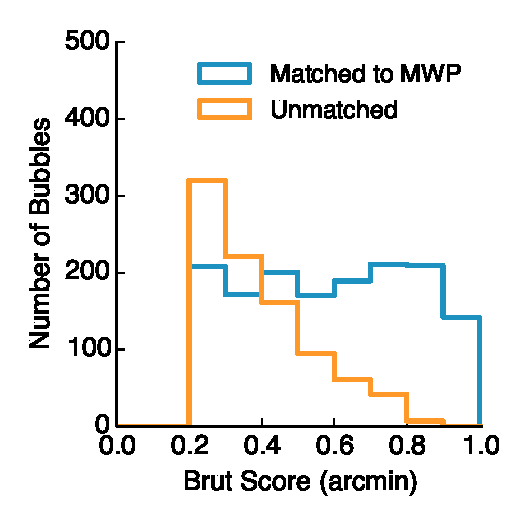
\includegraphics{new_score}
\caption{The distribution of Brut Scores for bubble candidates identified during the blind search.}
\label{fig:new_score}
\end{figure}

We can't rule out the possibility of bubbles missed by both Brut and the Milky Way Project -- it is possible, for example, that Brut could have learned a selection bias present in the training data. However, we conclude from this exercise that Brut's ability to identify bubble candidates in a blind search is comparable to citizen scientists, and such techniques can be useful as a way to pre-process large datasets. Furthermore, we note that the combined efforts of Brut and the MWP yield a much larger catalog of high-reliability bubbles than the previous catalogs curated by professional astronomers \citep{Churchwell06, Churchwell07}.

\begin{figure*}
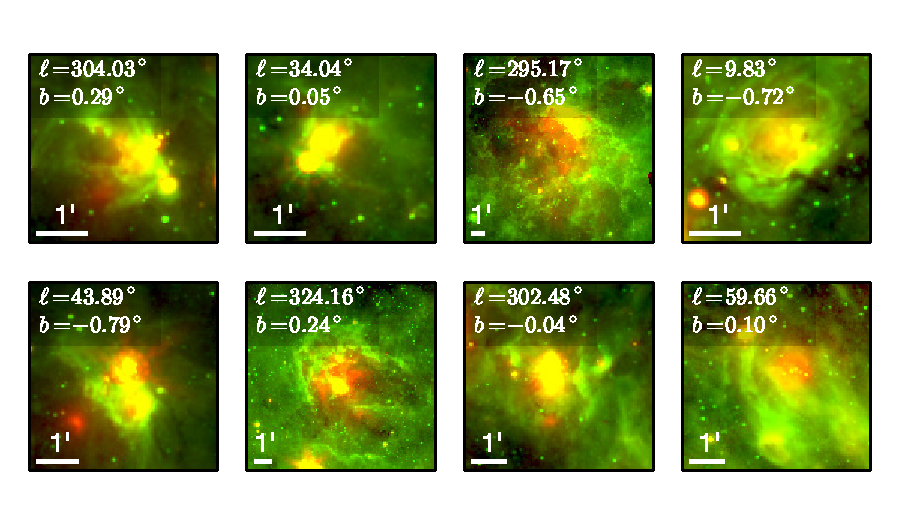
\includegraphics{new_gallery}
\caption{Eight bubbles not present in the Milky Way Project catalog, discovered by Brut during a blind search.}
\label{fig:new_gallery}
\end{figure*}

\section{Next Steps}
\label{sec:next_steps}
The success of Brut demonstrates the potential synergies that exist between machine learning, professional scientists, and citizen scientists. Note the complementary strengths and weaknesses of each resource:

\begin{enumerate}
\item Professional scientists are best-suited to perform nuanced classification tasks that require domain-specific knowledge. They are also the most resource-limited.
\item Citizen scientists outnumber professional scientists by orders of magnitude (in the case of Bubble detection, the factor is nearly 10,000:1). They are equally capable with the generic aspects of pattern recognition, but do not possess the domain expertise of professionals.
\item Supervised machine learning algorithms have no a-priori pattern recognition ability, and require external training. However, once supplied with this information, computer-driven analyses are reproducible and extremely scalable.
\end{enumerate}

Brut leverages the information provided by astronomers and citizen scientists alike. Citizen scientist input was used for training, and a smaller dataset of high-quality expert information set was used to convert Brut's classifications into calibrated bubble probabilities. The result is a classifier that is both more precise than the raw citizen scientist catalog, and more complete than the best expert-assembled catalog.

Searching \emph{Spitzer} images for bubbles is a small enough task that citizen scientists were able to perform an exhaustive search. Consequently, the MWP catalog appears to contain most of the bubbles that one can hope to identify from these images. Brut's main benefit is in providing an independent, probabilistic assessment of the MWP catalog, identifying interlopers in the catalog, and adding a small number of bubbles missed by citizen scientists -- particularly bubbles near bright objects.

However, one can hypothetically envision tools like Brut assisting professional and citizen scientists in real time. For searches for rarer objects in larger datasets, exhaustive human search is infeasible -- both due to boredom and prohibitive data sizes. Had Brut been trained at the start of the Milky Way Project, it would quickly have been able to eliminate many regions as devoid of bubbles. Citizen scientists could have spent more time classifying more ambiguous regions, which is where their input is most valuable (and where the tasks is likely most interesting). These ideas are explored in more depth by \cite{MSR}, and will become increasingly important as data continues to grow.

Similarly, Brut could easily incorporate additional sources of information. For example, far-infrared observations from \emph{Herschel} constrain the column density and temperature of dust in the vicinity of bubbles \citep{Anderson12}. This additional information can further disambiguate real bubbles from other cavities in the ISM. A followup investigation could supplement Brut's feature vectors with features extracted from \emph{Herschel} data, and retrain the classifiers. This is a promising approach to search for bubbles in the outer galaxy, since \emph{Spitzer} did not systematically survey the outer Galaxy at 8 or 24 \um\, and citizen scientists have not (yet) surveyed this region.


\section{Conclusion}
\label{sec:conclusion_ch6_brut}
We have developed an automatic bubble detector, Brut, using the Random Forest classification algorithm in tandem with a catalog of citizen scientist-identified bubbles in our galaxy. This algorithm is effective at detecting bubbles in \emph{Spitzer} images. By comparing the confidence scores that Brut computes with expert classifications of a small set of images, we are able to estimate the probability that any given region in \emph{Spitzer} {\sc glimpse} and {\sc mipsgal} data contains a bubble. We have used Brut to re-assess the objects in the Milky Way Project catalog, and also to perform a full search over {\sc glimpse} and {\sc mipsgal} images for new bubbles.  Several insights have emerged from this analysis:
\begin{enumerate}
\item Roughly 30\% of the objects in the Milky Way Project catalog are interlopers -- structures which a majority of experts would not consider to be likely \hii\, regions or wind blown bubbles.
\item Brut is able to identify which objects are probable interlopers, and likewise to identify highly probable bubbles. Compared to the MWP catalog as a whole, high-probability bubbles have a narrower latitude distribution, and are nearly 5 times more likely to be associated with \hii\, regions identified by \cite{Anderson11}.
\item The MWP catalog has a higher concentration of low-probability bubbles near giant \hii\, regions, which fluoresce the surrounding ISM and reveal more coincidental circular structures. Citizen scientists are prone to identify these regions as bubbles, whereas experts and Brut do not.
\item High probability bubbles  exhibit stronger excesses of YSOs and compact \hii\, regions along and interior to bubble rims -- a prediction of triggered star formation theories.
\end{enumerate}

Image classification remains a difficult problem in many contexts, and techniques like Brut are not yet as good as expert human analysis. However, Brut demonstrates that automated techniques are a valuable complement to manual search.  Combining human and machine searches is the most promising avenue for scaling tasks like astrophysical image classification to very large datasets.


\begin{thebibliography}{16}
\expandafter\ifx\csname natexlab\endcsname\relax\def\natexlab#1{#1}\fi

\bibitem[Anderson et al.(2011)]{Anderson11} Anderson, L.~D.,
Bania, T.~M., Balser, D.~S., \& Rood, R.~T.\ 2011, \apjs, 194, 32

\bibitem[Anderson et
al.(2012)]{Anderson12} Anderson, L.~D., Zavagno, A., Deharveng, L., et al.\ 2012, \aap, 542, A10

\bibitem[Arce et al.(2011)]{Arce11} Arce, H.~G., Borkin,
M.~A., Goodman, A.~A., Pineda, J.~E.,
\& Beaumont, C.~N.\ 2011, \apj, 742, 105

\bibitem[Beaumont
\& Williams(2010)]{Beaumont10} Beaumont, C.~N., \& Williams, J.~P.\ 2010, \apj, 709, 791

\bibitem[Beaumont et al.(2011)]{Beaumont11} Beaumont, C.~N.,
Williams, J.~P., \& Goodman, A.~A.\ 2011, \apj, 741, 14

\bibitem[Benjamin et al.(2003)]{Benjamin03} Benjamin, R.~A.,
Churchwell, E., Babler, B.~L., et al.\ 2003, \pasp, 115, 953

\bibitem[Bertoldi(1989)]{Bertoldi89} Bertoldi, F.\ 1989, \apj,
346, 735

\bibitem[Bradshaw et al.(2011)]{Bradshaw11} Bradshaw, E.~J.,
Almaini, O., Hartley, W.~G., et al.\ 2011, \mnras, 415, 2626

\bibitem[Breiman (2001)]{Breiman01} Breiman, Leo\ 2001, Machine Learning, 45, 5-32

\bibitem[Carey et al.(2009)]{Carey09} Carey, S.~J.,
Noriega-Crespo, A., Mizuno, D.~R., et al.\ 2009, \pasp, 121, 76

\bibitem[Castor et al.(1975)]{Castor75} Castor, J., McCray, R.,
\& Weaver, R.\ 1975, \apjl, 200, L107

\bibitem[Churchwell et al.(2006)]{Churchwell06} Churchwell, E.,
Povich, M.~S., Allen, D., et al.\ 2006, \apj, 649, 759

\bibitem[Churchwell et al.(2007)]{Churchwell07} Churchwell, E.,
Watson, D.~F., Povich, M.~S., et al.\ 2007, \apj, 670, 428

\bibitem[Dale et al.(2007)]{Dale07} Dale, J.~E., Bonnell,
I.~A., \& Whitworth, A.~P.\ 2007, \mnras, 375, 1291

\bibitem[Deharveng et
al.(2005)]{Deharveng05} Deharveng, L., Zavagno, A., \& Caplan, J.\ 2005, \aap, 433, 565

\bibitem[Everett
\& Churchwell(2010)]{Everett10} Everett, J.~E., \& Churchwell, E.\ 2010, \apj, 713, 592

\bibitem[Freyer et al.(2003)]{Freyer03} Freyer, T., Hensler, G.,
\& Yorke, H.~W.\ 2003, \apj, 594, 888

\bibitem[Helfand et al.(2006)]{Helfand06} Helfand, D.~J., Becker,
R.~H., White, R.~L., Fallon, A., \& Tuttle, S.\ 2006, \aj, 131, 2525

\bibitem[Hindson et al.(2012)]{Hindson12} Hindson, L., Thompson,
M.~A., Urquhart, J.~S., et al.\ 2012, \mnras, 421, 3418

\bibitem[Kamar et al.(2012)]{MSR} Kamar, Hacker, Severin, \& Horvitz, Eric\ 2012, Autonomous Agents and Multiagent Systems, 1, 467

\bibitem[Kendrew et al.(2012)]{Kendrew12} Kendrew, S., Simpson,
R., Bressert, E., et al.\ 2012, \apj, 755, 71

\bibitem[Koenig et al.(2008)]{Koenig08} Koenig, X.~P., Allen,
L.~E., Gutermuth, R.~A., et al.\ 2008, \apj, 688, 1142

\bibitem[Kuhn \& Johnson(2013)]{Kuhn13} Kuhn, Max, \& Johnson, Kjell\ 2013, \textit{Applied Predictive Modeling}, Springer

\bibitem[Lada
\& Lada(2003)]{Lada03} Lada, C.~J., \& Lada, E.~A.\ 2003, \araa, 41, 57

\bibitem[Landy
\& Szalay(1993)]{Landy93} Landy, S.~D., \& Szalay, A.~S.\ 1993, \apj, 412, 64

\bibitem[Matzner(2002)]{Matzner02} Matzner, C.~D.\ 2002, \apj,
566, 302

\bibitem[Mottram et
al.(2007)]{RMS} Mottram, J.~C., Hoare, M.~G., Lumsden, S.~L., et al.\ 2007, \aap, 476, 1019

\bibitem[Raddick et al.(2013)]{Raddick13} Raddick, J.~R., Bracey, G., Gay, P.~L. et al\ 2013, arXiv, 1303.6886

\bibitem[Rahman et al.(2011)]{Rahman11} Rahman, M., Matzner, C.,
\& Moon, D.-S.\ 2011, \apjl, 728, L37

\bibitem[Raileanu \& Kilian (2004)]{Raileanu04} Raileanu, L.~E. \& Stoffel, K.\ 2004, Annals of Mathematics and Artificial Intelligence, 41, 77

\bibitem[Robin et
al.(2003)]{Robin03} Robin, A.~C., Reyl{\'e}, C., Derri{\`e}re, S., \& Picaud, S.\ 2003, \aap, 409, 523

\bibitem[Robitaille et
al.(2012)]{Robitaille12} Robitaille, T.~P., Churchwell, E., Benjamin, R.~A., et al.\ 2012, \aap, 545, A39

\bibitem[Simpson et al.(2012)]{Simpson12} Simpson, R.~J., Povich,
M.~S., Kendrew, S., et al.\ 2012, \mnras, 424, 2442

\bibitem[Str{\"o}mgren(1939)]{Stromgren39} Str{\"o}mgren, B.\ 1939,
\apj, 89, 526

\bibitem[Thompson et al.(2012)]{Thompson12} Thompson, M.~A.,
Urquhart, J.~S., Moore, T.~J.~T., \& Morgan, L.~K.\ 2012, \mnras, 421, 408

\bibitem[Tola et al. (2010)]{DAISY}Tola Engin, Lepetit, V. \& Fua, P.\ 2010, IEEE Transactions on Pattern Analysis and Machine Intelligence, 32, 5, 815-830

\bibitem[Viola \& Jones (2001)]{ViolaJones}Viola, Paul, \& Jones,\ 2001, Proceedings of the 2001 IEEE Computer Society Conference on Computer Vision and Pattern Recognition, 1, I-511

\bibitem[Weaver et al.(1977)]{Weaver77} Weaver, R., McCray, R.,
Castor, J., Shapiro, P., \& Moore, R.\ 1977, \apj, 218, 377

\bibitem[Whitworth et al.(1994)]{Whitworth94} Whitworth, A.~P.,
Bhattal, A.~S., Chapman, S.~J., Disney, M.~J.,
\& Turner, J.~A.\ 1994, \mnras, 268, 291

\bibitem[Zavagno et
al.(2006)]{Zavagno06} Zavagno, A., Deharveng, L., Comer{\'o}n, F., et al.\ 2006, \aap, 446, 171

\bibitem[Zhang \& Zhang (2010)]{Zhang10}Zhang, C., \& Zhang, Z.\ 2010, A survey of recent advances in face detection, Technical Report, Microsoft Research

\bibitem[Zinnecker
\& Yorke(2007)]{Zinnecker07} Zinnecker, H., \& Yorke, H.~W.\ 2007, \araa, 45, 481

\end{thebibliography}

\section{Appendix A: Expert Survey}
Figure \ref{fig:expert_form} shows the interface experts used to provide classifications for the expert survey. Each object is shown 6 times, at 3 zoom levels (columns) and two contrast settings (rows). Experts were asked to click one of the three buttons to classify the object as a non-bubble, ambiguous/irregular bubble, or clear bubble. To minimize the effects of fatigue, each user classified objects in a different, random order.

Figure \ref{fig:mwp_survey_gallery} shows the objects in the survey that were drawn randomly from the Milky Way Project catalog. Each image corresponds to the upper-left image of the survey form. Similarly, Figure \ref{fig:uniform_survey_gallery} shows the objects in the uniform sample. Recall that these were selected to be uniformly distributed in Brut's confidence score.


\begin{figure}
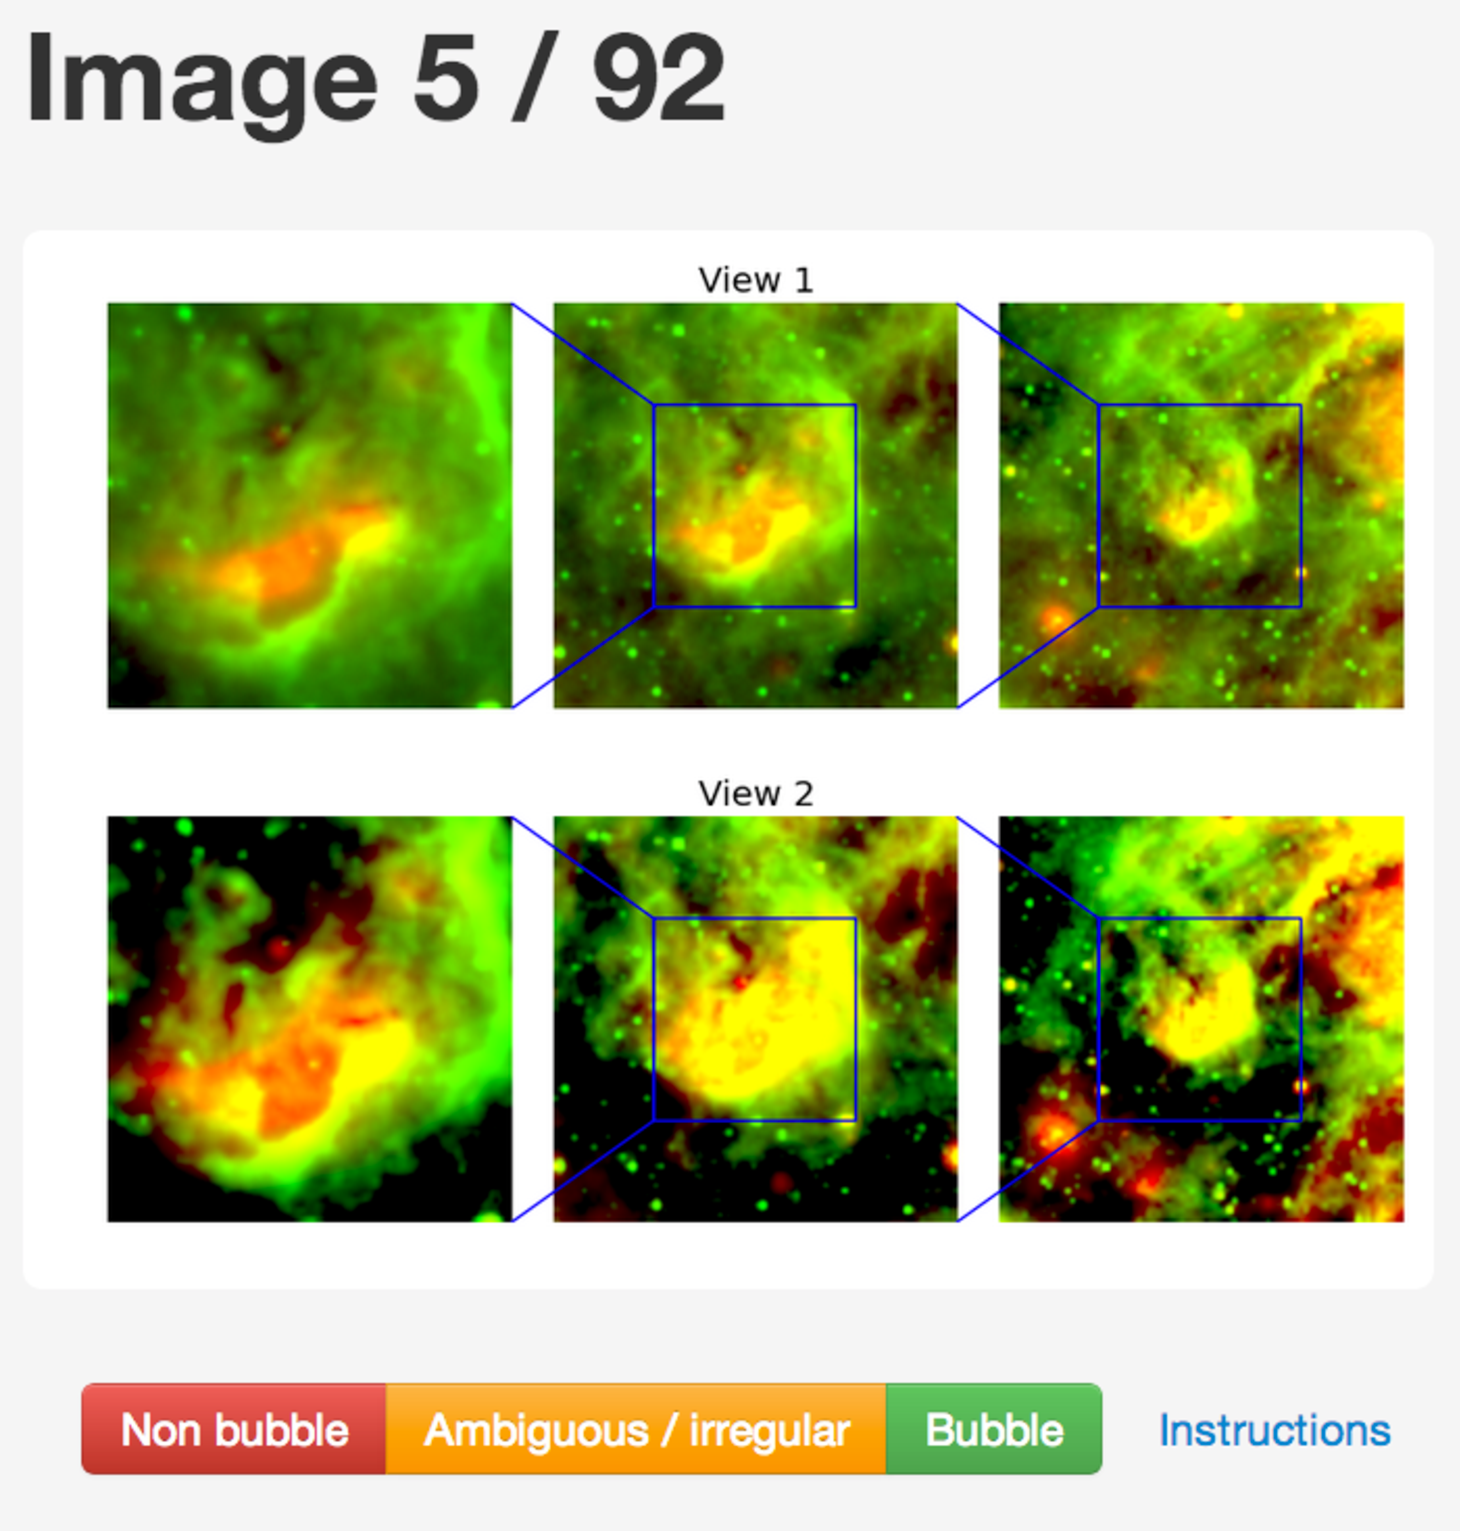
\includegraphics[width=5in]{expert_form}
\caption{A page from the expert survey, showing a possible bubble at 3 zoom levels and 2 contrast settings.}
\label{fig:expert_form}
\end{figure}


\begin{figure}
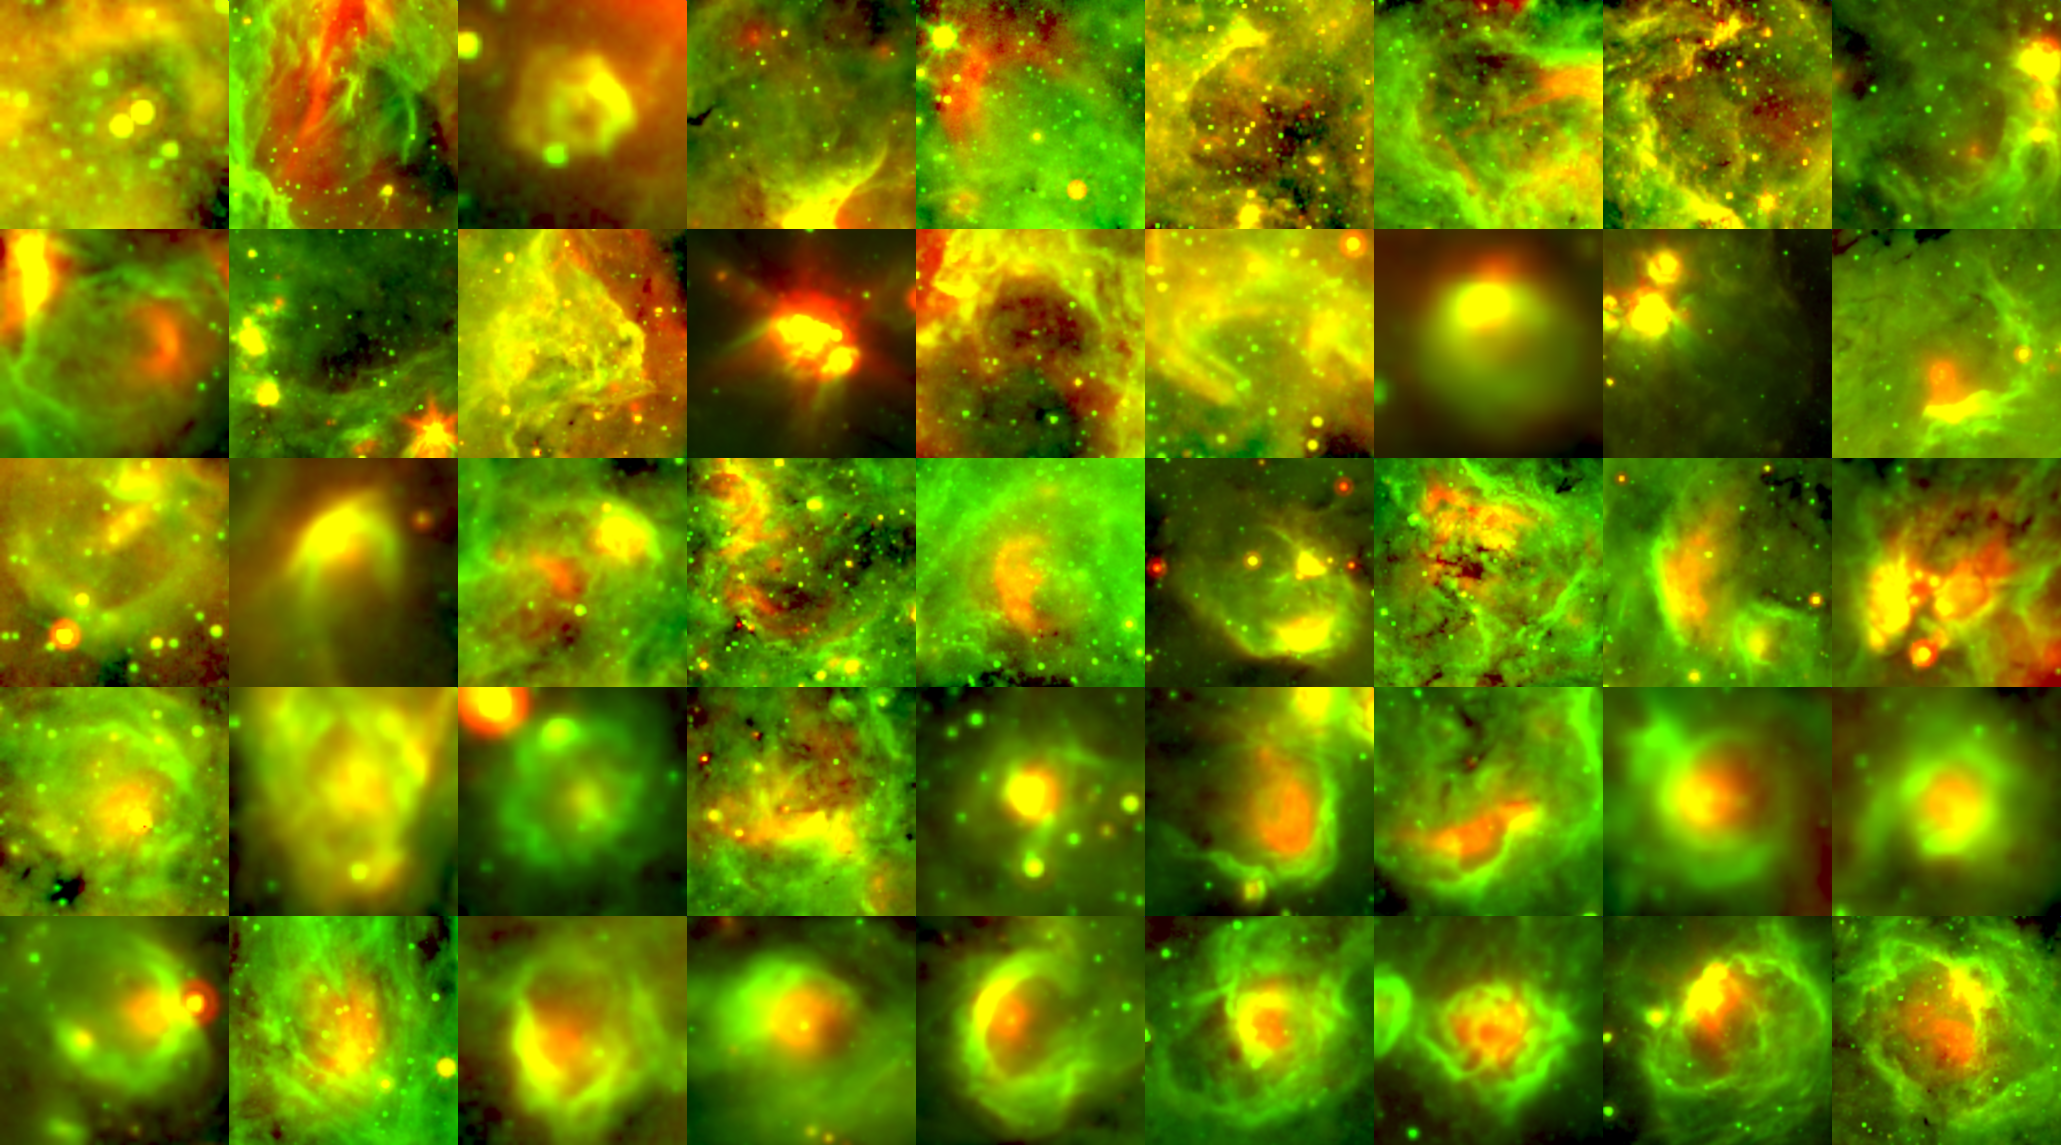
\includegraphics[width=6in]{mwp_survey_gallery}
\caption{The objects in the expert survey selected from the Milky Way Project catalog. Objects are sorted by Brut's confidence score.}
\label{fig:mwp_survey_gallery}
\end{figure}

\begin{figure}
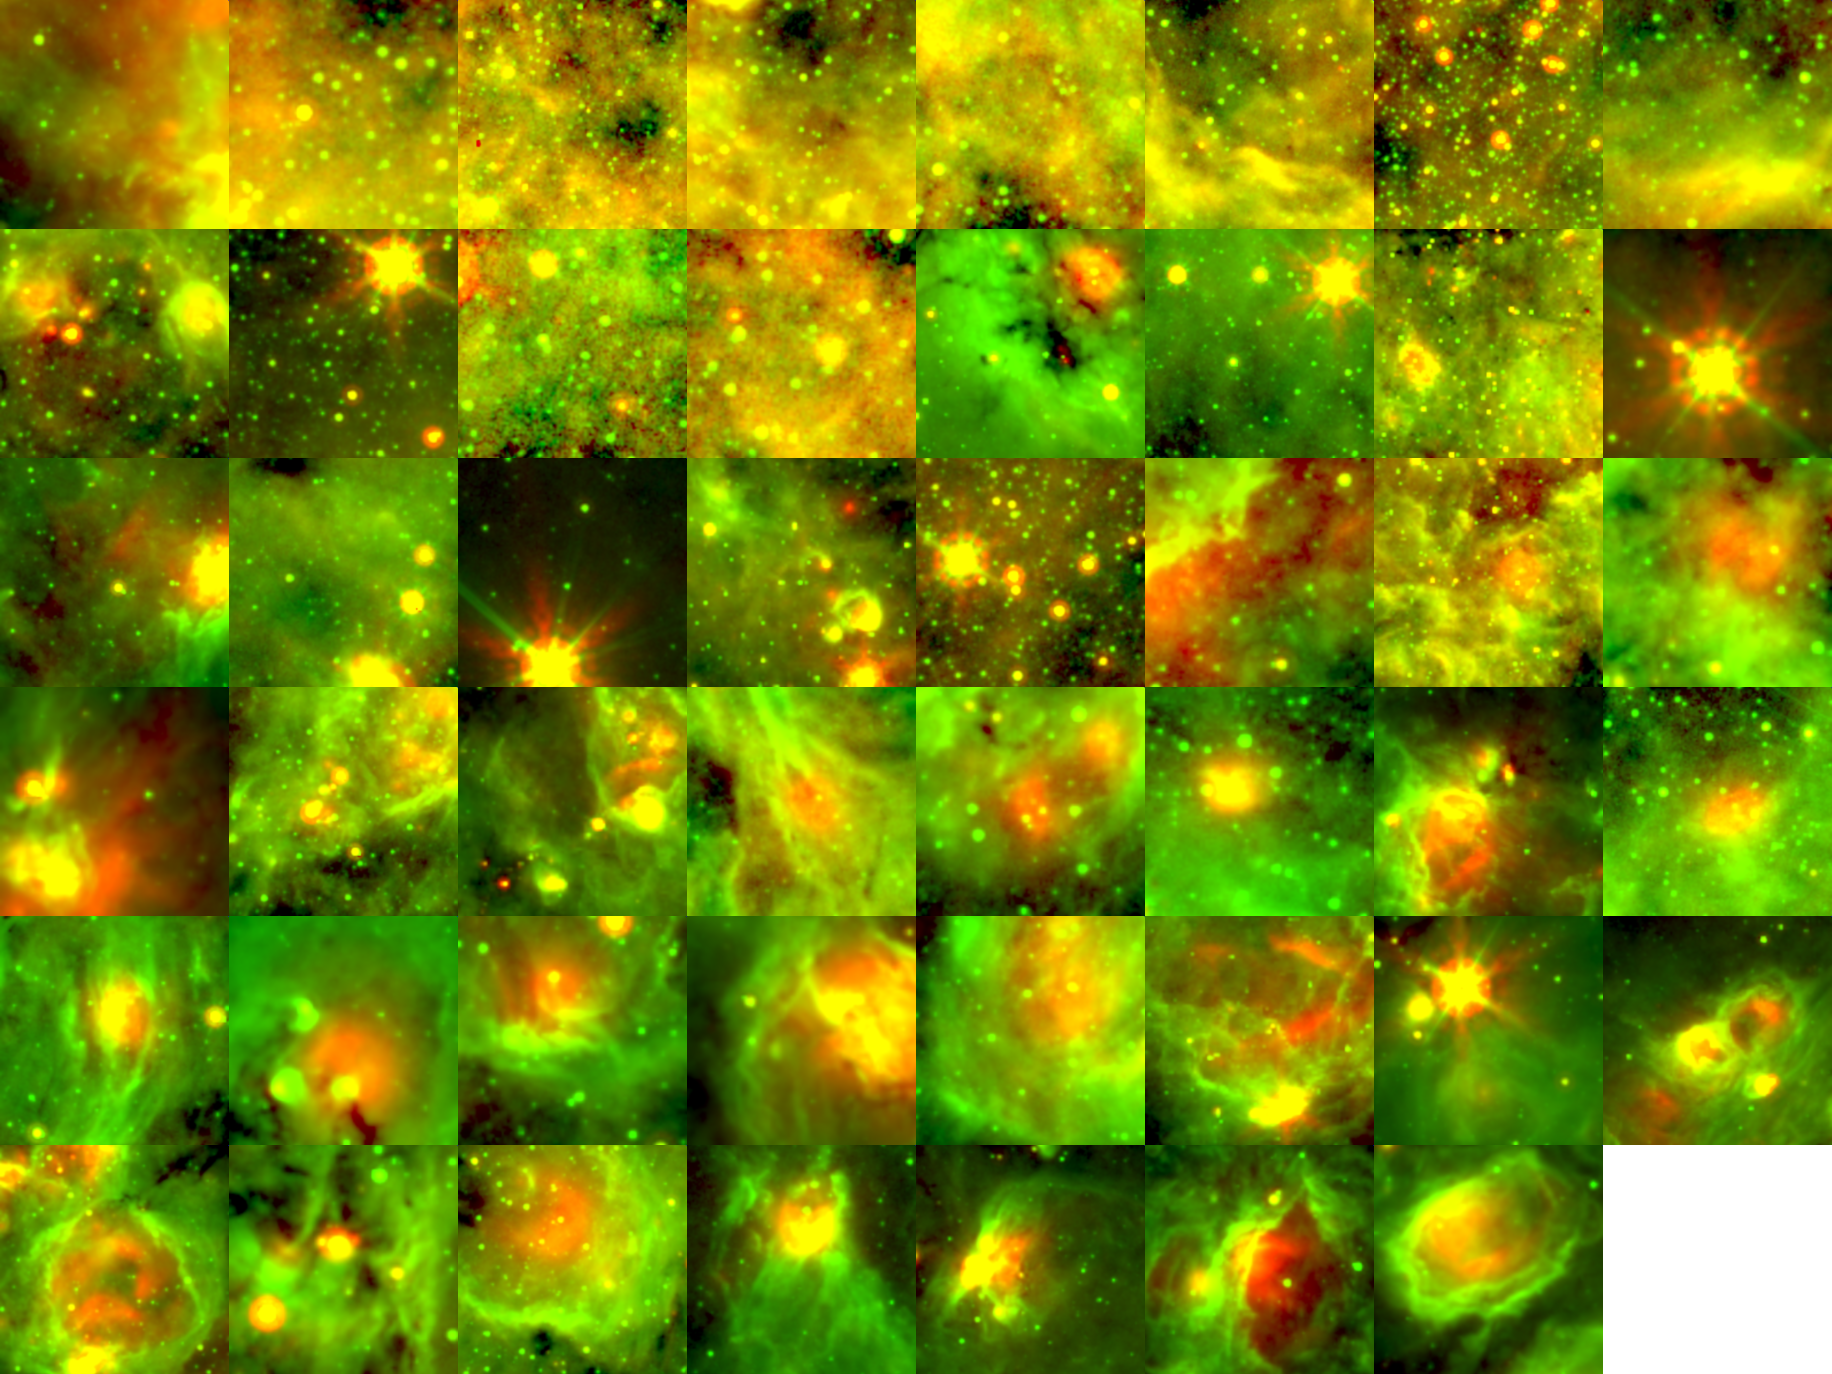
\includegraphics[width=6in]{uniform_survey_gallery}
\caption{The same as Figure \ref{fig:mwp_survey_gallery}, but for objects from the uniform sample.}
\label{fig:uniform_survey_gallery}
\end{figure}

\cfinput{prob_table_head.tex}
